%  LaTeX support: latex@mdpi.com 
%  For support, please attach all files needed for compiling as well as the log file, and specify your operating system, LaTeX version, and LaTeX editor.

%=================================================================
\documentclass[mathematics,article,accept,pdftex,moreauthors]{Definitions/mdpi} 
% For posting an early version of this manuscript as a preprint, you may use "preprints" as the journal and change "submit" to "accept". The document class line would be, e.g., \documentclass[preprints,article,accept,moreauthors,pdftex]{mdpi}. This is especially recommended for submission to arXiv, where line numbers should be removed before posting. For preprints.org, the editorial staff will make this change immediately prior to posting.

%--------------------
% Class Options:
%--------------------
%----------
% journal
%----------
% Choose between the following MDPI journals:
% acoustics, actuators, addictions, admsci, adolescents, aerospace, agriculture, agriengineering, agronomy, ai, algorithms, allergies, alloys, analytica, animals, antibiotics, antibodies, antioxidants, applbiosci, appliedchem, appliedmath, applmech, applmicrobiol, applnano, applsci, aquacj, architecture, arts, asc, asi, astronomy, atmosphere, atoms, audiolres, automation, axioms, bacteria, batteries, bdcc, behavsci, beverages, biochem, bioengineering, biologics, biology, biomass, biomechanics, biomed, biomedicines, biomedinformatics, biomimetics, biomolecules, biophysica, biosensors, biotech, birds, bloods, blsf, brainsci, breath, buildings, businesses, cancers, carbon, cardiogenetics, catalysts, cells, ceramics, challenges, chemengineering, chemistry, chemosensors, chemproc, children, chips, cimb, civileng, cleantechnol, climate, clinpract, clockssleep, cmd, coasts, coatings, colloids, colorants, commodities, compounds, computation, computers, condensedmatter, conservation, constrmater, cosmetics, covid, crops, cryptography, crystals, csmf, ctn, curroncol, currophthalmol, cyber, dairy, data, dentistry, dermato, dermatopathology, designs, diabetology, diagnostics, dietetics, digital, disabilities, diseases, diversity, dna, drones, dynamics, earth, ebj, ecologies, econometrics, economies, education, ejihpe, electricity, electrochem, electronicmat, electronics, encyclopedia, endocrines, energies, eng, engproc, ent, entomology, entropy, environments, environsciproc, epidemiologia, epigenomes, est, fermentation, fibers, fintech, fire, fishes, fluids, foods, forecasting, forensicsci, forests, foundations, fractalfract, fuels, futureinternet, futureparasites, futurepharmacol, futurephys, futuretransp, galaxies, games, gases, gastroent, gastrointestdisord, gels, genealogy, genes, geographies, geohazards, geomatics, geosciences, geotechnics, geriatrics, hazardousmatters, healthcare, hearts, hemato, heritage, highthroughput, histories, horticulturae, humanities, humans, hydrobiology, hydrogen, hydrology, hygiene, idr, ijerph, ijfs, ijgi, ijms, ijns, ijtm, ijtpp, immuno, informatics, information, infrastructures, inorganics, insects, instruments, inventions, iot, j, jal, jcdd, jcm, jcp, jcs, jdb, jeta, jfb, jfmk, jimaging, jintelligence, jlpea, jmmp, jmp, jmse, jne, jnt, jof, joitmc, jor, journalmedia, jox, jpm, jrfm, jsan, jtaer, jzbg, kidney, kidneydial, knowledge, land, languages, laws, life, liquids, literature, livers, logics, logistics, lubricants, lymphatics, machines, macromol, magnetism, magnetochemistry, make, marinedrugs, materials, materproc, mathematics, mca, measurements, medicina, medicines, medsci, membranes, merits, metabolites, metals, meteorology, methane, metrology, micro, microarrays, microbiolres, micromachines, microorganisms, microplastics, minerals, mining, modelling, molbank, molecules, mps, msf, mti, muscles, nanoenergyadv, nanomanufacturing, nanomaterials, ncrna, network, neuroglia, neurolint, neurosci, nitrogen, notspecified, nri, nursrep, nutraceuticals, nutrients, obesities, oceans, ohbm, onco, oncopathology, optics, oral, organics, organoids, osteology, oxygen, parasites, parasitologia, particles, pathogens, pathophysiology, pediatrrep, pharmaceuticals, pharmaceutics, pharmacoepidemiology, pharmacy, philosophies, photochem, photonics, phycology, physchem, physics, physiologia, plants, plasma, pollutants, polymers, polysaccharides, poultry, powders, preprints, proceedings, processes, prosthesis, proteomes, psf, psych, psychiatryint, psychoactives, publications, quantumrep, quaternary, qubs, radiation, reactions, recycling, regeneration, religions, remotesensing, reports, reprodmed, resources, rheumato, risks, robotics, ruminants, safety, sci, scipharm, seeds, sensors, separations, sexes, signals, sinusitis, skins, smartcities, sna, societies, socsci, software, soilsystems, solar, solids, sports, standards, stats, stresses, surfaces, surgeries, suschem, sustainability, symmetry, synbio, systems, taxonomy, technologies, telecom, test, textiles, thalassrep, thermo, tomography, tourismhosp, toxics, toxins, transplantology, transportation, traumacare, traumas, tropicalmed, universe, urbansci, uro, vaccines, vehicles, venereology, vetsci, vibration, viruses, vision, waste, water, wem, wevj, wind, women, world, youth, zoonoticdis 

%---------
% article
%---------
% The default type of manuscript is "article", but can be replaced by: 
% abstract, addendum, article, book, bookreview, briefreport, casereport, comment, commentary, communication, conferenceproceedings, correction, conferencereport, entry, expressionofconcern, extendedabstract, datadescriptor, editorial, essay, erratum, hypothesis, interestingimage, obituary, opinion, projectreport, reply, retraction, review, perspective, protocol, shortnote, studyprotocol, systematicreview, supfile, technicalnote, viewpoint, guidelines, registeredreport, tutorial
% supfile = supplementary materials

%----------
% submit
%----------
% The class option "submit" will be changed to "accept" by the Editorial Office when the paper is accepted. This will only make changes to the frontpage (e.g., the logo of the journal will get visible), the headings, and the copyright information. Also, line numbering will be removed. Journal info and pagination for accepted papers will also be assigned by the Editorial Office.

%------------------
% moreauthors
%------------------
% If there is only one author the class option oneauthor should be used. Otherwise use the class option moreauthors.

%---------
% pdftex
%---------
% The option pdftex is for use with pdfLaTeX. If eps figures are used, remove the option pdftex and use LaTeX and dvi2pdf.

%=================================================================
% MDPI internal commands
\firstpage{1} 
\makeatletter 
\setcounter{page}{\@firstpage} 
\makeatother
\pubvolume{1}
\issuenum{1}
\articlenumber{0}
\pubyear{2022}
\copyrightyear{2022}
\externaleditor{{Academic Editors: Theodore E. Simos and Charampos Tsitouras}} 
\datereceived{6 July 2022} 
%\daterevised{} % Only for the journal Acoustics
\dateaccepted{28 July 2022} 
\datepublished{} 
%\datecorrected{} % Corrected papers include a "Corrected: XXX" date in the original paper.
%\dateretracted{} % Corrected papers include a "Retracted: XXX" date in the original paper.
\hreflink{https://doi.org/} % If needed use \linebreak
%\doinum{}
%------------------------------------------------------------------
% The following line should be uncommented if the LaTeX file is uploaded to arXiv.org
%\pdfoutput=1

%=================================================================
% Add packages and commands here. The following packages are loaded in our class file: fontenc, inputenc, calc, indentfirst, fancyhdr, graphicx, epstopdf, lastpage, ifthen, lineno, float, amsmath, setspace, enumitem, mathpazo, booktabs, titlesec, etoolbox, tabto, xcolor, soul, multirow, microtype, tikz, totcount, changepage, attrib, upgreek, cleveref, amsthm, hyphenat, natbib, hyperref, footmisc, url, geometry, newfloat, caption

%=================================================================
%% Please use the following mathematics environments: Theorem, Lemma, Corollary, Proposition, Characterization, Property, Problem, Example, ExamplesandDefinitions, Hypothesis, Remark, Definition, Notation, Assumption
%% For proofs, please use the proof environment (the amsthm package is loaded by the MDPI class).

%=================================================================
% Full title of the paper (Capitalized)
\Title{Optimization of Turbulence Model Parameters Using the Global Search Method Combined with Machine Learning}
% MDPI: 
%Notes for authors:
%Please carefully check the accuracy of names and affiliations. Please note that authorship CAN NOT be changed.
% 1. The paper was edited by our English editor, please check the whole text and confirm if your meaning is retained.
%2. Do not delete any comment we left for you and reply to each comment so that we can understand your meaning clearly.
%3. If you need to revise somewhere in your paper, please highlight the revisions to make us known.
%4. Please check if there are duplicated equations, if yes, please revise
%5. Please make sure that all the symbols in the paper are of the same format.
%(Thank you for your cooperation in advance.)
% MDPI internal command: Title for citation in the left column
\TitleCitation{Optimization of Turbulence Model Parameters Using the Global Search Method Combined with Machine Learning}

% Author Orchid ID: enter ID or remove command
\newcommand{\orcidauthorA}{0000-0001-5273-2471} % Add \orcidA{} behind the author's name
\newcommand{\orcidauthorB}{0000-0002-8736-0652} % Add \orcidB{} behind the author's name
\newcommand{\orcidauthorC}{0000-0002-0722-6884} % Add \orcidC{} behind the author's name

\newcommand{\orcidauthorD}{0000-0002-5771-4114} % Add \orcidD{} behind the author's name
\newcommand{\orcidauthorE}{0000-0001-5525-5180} % Add \orcidF{} behind the author's name
\newcommand{\orcidauthorF}{0000-0001-9568-7121} % Add \orcidG{} behind the author's name

% Authors, for the paper (add full first names)
%\Author{Firstname Lastname $^{1,\dagger,\ddagger}$\orcidA{}, Firstname Lastname $^{2,\ddagger}$ and Firstname Lastname $^{2,}$*}
\Author{Константин Баркалов $^{1}$\orcidA{}, Илья Лебедев $^{1}$\orcidB{}, Марина Усова $^{1}$\orcidC{}, Дарья Романова $^{{2},{3}}$\orcidD{}, Даниил Рязанов $^2$\orcidF{} \mbox{и Сергей Стрижак} $^{2,{4},}$*\orcidE{}} 
%MDPI: 1. Please carefully check the accuracy of names and affiliations. 
%Authors: Names and affilations are correct
%MDPI: 2. Affiliations should mentioned in order, we have revised the affiliation number, please confirm. 
%Authors: Ok
%MDPI: 3. please check if the orcid of author  Marina Usova is correct
%Authors: Yes, it is correct

%\longauthorlist{yes}

% MDPI internal command: Authors, for metadata in PDF
%\AuthorNames{Firstname Lastname, Firstname Lastname and Firstname Lastname}
\AuthorNames{Константин Баркалов, Илья Лебедев, Марина Усова, Дарья Романова, Даниил Рязанов и Сергей Стрижак}

% MDPI internal command: Authors, for citation in the left column
%\AuthorCitation{Lastname, F.; Lastname, F.; Lastname, F.}
\AuthorCitation{Barkalov, K.; %MDPI: Please carefully check the accuracy of names.
%Authors: Checked
 Lebedev, I.; Usova, M.; Romanova, D.; Ryazanov, D.; Strijhak, S.}
% If this is a Chicago style journal: Lastname, Firstname, Firstname Lastname, and Firstname Lastname.

% Affiliations / Addresses (Add [1] after \address if there is only one affiliation.)
%\address{%
%$^{1}$ \quad Affiliation 1; e-mail@e-mail.com\\
%$^{2}$ \quad Affiliation 2; e-mail@e-mail.com}
\address{%
$^{1}$ \quad Кафедра математического обеспечения и суперкомпьютерных технологий, ННГУ им. Н.И. Лобачевского, 603022~Нижний Новгород, Россия; konstantin.barkalov@itmm.unn.ru (K.B.); ilya.lebedev@itmm.unn.ru (I.L.); usova@itmm.unn.ru (M.U.)\\
%MDPI: The email of this author is different from the submitting system(usova@itmm.unn.ru). Please confirm which one is correct.
%Authors: Fixed to correct one

$^{2}$ \quad Институт системного программирования им. В.П. Иванникова РАН,  
%MDPI: Please check if it should be revised to ``Ivannikov Institute for System Programming, Russian Academy of Sciences''
%Authors: Corrected
 109004~Москва, Россия; romanovadi@ispras.ru (D.R.) ryazanov@ispras.ru (D.R.) \\
$^{3}$ \quad Механико-математический факультет МГУ имени М.В. Ломоносова, 119991~Москва, Россия  \\
%MDPI: newly added  department based on his published paper in MDPI, please confirm if it is correct.
%Authors: Yes, it is correct
$^{4}$ \quad Московский авиационный институт, 125993~Москва, Россия 
%MDPI: We rearranged addresses information, please confirm
%Authors: Ok
}


% Contact information of the corresponding author
%\corres{Correspondence: e-mail@e-mail.com; Tel.: (optional; include country code; if there are multiple corresponding authors, add author initials) +xx-xxxx-xxx-xxxx (F.L.)}
\corres{Correspondence: s.strijhak@ispras.ru}

% Current address and/or shared authorship
%\firstnote{Current address: Affiliation 3.} 
%\secondnote{These authors contributed equally to this work.}
% The commands \thirdnote{} till \eighthnote{} are available for further notes

%\simplesumm{} % Simple summary

%\conference{} % An extended version of a conference paper

% Abstract (Do not insert blank lines, i.e., \\) 
\abstract{В статье рассматривается проблема нахождения оптимальных значений параметров математической модели на примере расчёта склонового течения. Склоновое течение моделируется с помощью метода конечных объемов, примененного к осредненным по Рейнольдсу уравнениям Навье–Стокса с замыканием в виде $k{-}\omega\ SST$
модели турбулентности. С помощью алгоритма глобального поиска найдены оптимальные значения коэффициентов модели турбулентности для гравитационных многофазных течений со свободной поверхностью. Калибровка проводилась для повышения сходства экспериментальных и расчетных профилей скорости. В качестве целевой функции в задаче оптимизации рассматривается среднеквадратическая ошибка (RMSE) между расчетным профилем скорости потока и экспериментальным профилем. Калибровка коэффициентов модели турбулентности для расчета течений со свободной поверхностью на наклонной поверхности с использованием многофазной модели для отслеживани интерфейса ранее не проводилась. Для решения задачи многопараметрической оптимизации, возникающей при поиске минимума функции потерь, мы применяем новый подход к оптимизации с использованием кривой Пеано для уменьшения размерности задачи. Для ускорения процедуры оптимизации целевая функция была аппроксимирована с помощью искусственной нейронной сети. Таким образом, был применен междисциплинарный подход, позволивший найти оптимальные значения шести параметров модели турбулентности с помощью программ OpenFOAM и Globalizer.}  
%MDPI: Please state the software version number, creator, and the location (city, country) from where the software was sourced.
%Authors: This information added in section 4.

% Keywords
\keyword{global optimization; artificial neural network; function approximation; finite volume method; CFD; OpenFOAM; interFoam} 

% The fields PACS, MSC, and JEL may be left empty or commented out if not applicable
%\PACS{J0101}
\MSC{62M45; 76D05; 76F60; 90C26} 
%MDPI: Please confirm MSC
%\JEL{}

%%%%%%%%%%%%%%%%%%%%%%%%%%%%%%%%%%%%%%%%%%
% Only for the journal Diversity
%\LSID{\url{http://}}

%%%%%%%%%%%%%%%%%%%%%%%%%%%%%%%%%%%%%%%%%%
% Only for the journal Applied Sciences
%\featuredapplication{Authors are encouraged to provide a concise description of the specific application or a potential application of the work. This section is not mandatory.}
%%%%%%%%%%%%%%%%%%%%%%%%%%%%%%%%%%%%%%%%%%

%%%%%%%%%%%%%%%%%%%%%%%%%%%%%%%%%%%%%%%%%%
% Only for the journal Data
%\dataset{DOI number or link to the deposited data set if the data set is published separately. If the data set shall be published as a supplement to this paper, this field will be filled by the journal editors. In this case, please submit the data set as a supplement.}
%\datasetlicense{License under which the data set is made available (CC0, CC-BY, CC-BY-SA, CC-BY-NC, etc.)}

%%%%%%%%%%%%%%%%%%%%%%%%%%%%%%%%%%%%%%%%%%
% Only for the journal Toxins
%\keycontribution{The breakthroughs or highlights of the manuscript. Authors can write one or two sentences to describe the most important part of the paper.}

%%%%%%%%%%%%%%%%%%%%%%%%%%%%%%%%%%%%%%%%%%
% Only for the journal Encyclopedia
%\encyclopediadef{For entry manuscripts only: please provide a brief overview of the entry title instead of an abstract.}

\usepackage{nomencl}
\makenomenclature

%%%%%%%%%%%%%%%%%%%%%%%%%%%%%%%%%%%%%%%%%%
\begin{document}

\section{Введение}

Изменение климата сопровождается опасными природными явлениями, которые становятся все более частыми. Эти явления неизбежно влияют на жизнь и повседневную деятельность человека. Исследование этих вопросов связано с математическим моделированием и анализом геофизических данных, а также данных численных и натурных экспериментов. Современная тенденция в анализе геоданных связана с использованием алгоритмов машинного обучения и искусственных нейронных сетей.

Оползни, сели и лавины относятся к опасным геологическим процессам. Они являются склоновыми процессами, связанными с отрывом горных пород, перемещением их по склону под влиянием силы тяжести и приводящим к необратимым преобразованиям в рельефе. Проблема изучения схода оползней, селей и лавин, их предсказания и обнаружения является актуальной задачей в связи с влиянием этого опасного явления на жизнь людей и городскую инфраструктуру. Оползни различают по основным причинам возникновения. Они бывают абразионные, эрозионные, техногенные и естественно-техногенные. По механизму смещения различают соответственно оползни блоковые, сдвига, растяжения, разжижения~\cite{Pendin2015}.

Данные показывают, что в период с января 2004 г. по декабрь 2016 г. оползни унесли жизни около 56 000 человек в 5 000 происшествий. Пространственное распределение оползней неравномерно, при этом преобладающим географическим регионом является Азия~\cite{Froude2018}.

Большое количество оползней, лавин и селей происходит в европейских странах (Швейцария, Австрия, Италия, Франция, Исландия). Подобные опасные явления имеют место и в России, например, в Краснодарском крае РФ и на Северном Кавказе, в связи с обильными осадками в этих районах, где присутствует горный рельеф, и в связи со стихийной застройкой территории (линейные и площадные объекты) в последние годы~\cite{hungr2005landslide}. На вышеуказанных территориях России (Сочи, Красная Поляна) в 2021 г. выпало выпадающее количество осадков. Это привело к разливу горных рек и увеличило опасность склоновых стоков. Произошли катастрофические сходы селей, приведшие к повреждению дорожной техники и перекрытию проезжей части~\cite{Harch2020}.

Селевые потоки являются одним из наиболее сложных экзогенных геологических процессов, интегрирующих действия других геологических процессов. Селевой поток -- это сложная гетерогенная структура, состоящая из жидкого и твердого компонентов. Твердый элемент состоит из неоднородных в гранулометрическом отношении минеральных частиц.

%Самая известная проблема оползня связана с оценкой устойчивости оползневого склона к статическим условиям и сейсмическому воздействию. Моделирование спуска склонового потока позволяет прогнозировать вызванные этим явлением разрушения, правильно размещать защитные сооружения и жизненно важные объекты.

Наиболее известная задача с оползнем связана с оценкой устойчивости оползневого склона для статических условий и сейсмического воздействия. Моделирование спуска склонового потока позволяет прогнозировать ущерб от этого явления и правильно размещать защитные сооружения и жизненно важные объекты. Такие задачи решаются с использованием метода конечных разностей~\cite{Bernander2016}, метода конечных объемов~\cite{liu2007application}, метода дискретных элементов~\cite{Liu2020}, метода клеточных автоматов ~\cite{piegari2006cellular} и гибридных методов. Селевые потоки можно смоделировать с помощью двухжидкостной модели, в основе которой используется модель объема в жидкости – Volume of Fluid~\cite{Hirt1981}. Перечисленные выше методы реализованы в различных коммерческих и открытых программных пакетах MN2D~\cite{Naaim2002}, TITAN2D~\cite{Pitman2003} и RAMMS.

Ранее изучение лавин проводилось методами вычислительной гидродинамики для ньютоновских жидкостей и анализа данных наблюдений, в том числе исторических данных о лавинах в Японии~\cite{Oda2011, Yamaguchi2017}. Аналогичные работы проводились с лавинами в Швейцарии, Австрии и Италии. В Исландском университете ~\cite{IceThesKatr, IceThesJon} проведена серия работ по изучению лавин с использованием лабораторного эксперимента в специальных лотках и измерительного оборудования для изучения лавин в Исландии. Эксперимент со спуском снежно-водяного потока в Давосе, Швейцария, описан в~\cite{Jaedicke2006}. Проведены измерения глубины потока для сухой снежной лавины и для снегово-водяного потока.

Чэн и др.~\cite{Cheung2011} использовали байесовский анализ для калибровки коэффициентов модели турбулентности Spalart--Allmaras, чтобы исправить недостатки модели и воспроизвести профиль турбулентного пограничного слоя над плоской пластиной. Среди подобных работ уже была проведена калибровка коэффициентов в $k-\varepsilon$ модели турбулентности при изучении процесса распространения примесей в процессе городской застройки~\cite{Guillas2014}.

Байесовский анализ часто используется для калибровки моделей турбулентности замыканий RANS для повышения точности прогноза без потери вычислительной эффективности (как это было сделано для модели $k{-}\varepsilon$ с функциями демпфирования Лаундера-Шармы, $k{-}\omega$ Wilcox-модели, Spalart--Allmaras и Baldwin--Lomax~\cite{Edeling2014a,Edeling2014b} моделей). Де Зордо-Банлиат и др. применил байесовский анализ к каскадам компрессоров, чтобы получить набор калиброванных параметров модели турбулентности из-за неадекватности исходной модели~\cite{deZordoBanliat2020}.

Котаро Мацуи и др.~\cite{Matsui2021} предложили новый набор калиброванных коэффициентов, которые улучшили способность модели Спаларта--Аллмараса прогнозировать угловое разделение потока в каскаде компрессора. Всесторонний обзор неопределенностей модели турбулентности дан в статье Сяо и Циннелла~\cite{Xiao2019}.

Всесторонний анализ климатических, геологических и гидрологических данных применялся для моделирования и прогнозирования склоновых стоков. В рамках последних тенденций огромные потоки данных, получаемых со спутников, из экспериментов и из математического моделирования, обрабатываются с помощью машинного обучения, что позволяет разрабатывать эффективные модели этих процессов~\cite{GeoML, Ma2020}.

%%%%% рецензент 2 начала цитирования

Недавно было предложено несколько новых методов оптимизации и машинного обучения.
В~\cite{YuWuWang2022} был предложен новый метод анализа сожалений, названный стохастической p-робастной оптимизацией, который позволяет одновременно использовать преимущества методов стохастической оптимизации и робастной оптимизации для изучения оптимальной работы гибридной энергетической системы.

Основанный на обучении метод создания аватаров в полный рост с учетом сигналов водителя был представлен в~\cite{BagautdnovWuSimon2021}. Модель представляла собой условный вариационный автокодер, который можно было анимировать с помощью неполных управляющих сигналов, таких как поза человека и ключевые точки лица, и производил высококачественное представление геометрии человека и внешнего вида в зависимости от вида.

В~\cite{ZhangZhangCai2022} была предложена новая многоклассовая стратегия диагностики неисправностей подшипников ветряных турбин, основанная на модели условно-вариационной генеративно-состязательной сети, сочетающей слияние сигналов из нескольких источников. Стратегия преобразовывала одномерные сигналы вибрации от нескольких источников в двумерные сигналы, а двумерные сигналы от нескольких источников объединялись с помощью вейвлет-преобразования.

Противоборствующая сеть с дополнительными метками (CLARINET) была предложена для решения проблем полностью комплементарной неконтролируемой адаптации домена (CC-UDA) и частично комплементарной неконтролируемой адаптации домена (PC-UDA). CLARINET одновременно поддерживает две глубокие сети, одна из которых занимается классификацией исходных данных с дополнительными метками, а другая занимается адаптацией распределения от источника к целевому~\cite{ZhangLiuFang2021}.

В~\cite{ZhongFangLiu2021} была рассмотрена сложная проблема, называемая неконтролируемой адаптацией домена с открытым набором (UOSDA). Авторы предложили практическую теоретическую границу для UOSDA, которая содержала эффективную оценку риска на данных с неизвестными классами. Кроме того, был предложен метод UOSDA на основе DNN под руководством предложенной теоретической оценки. Метод может точно оценить риск классификатора на данных с неизвестными классами и адекватно согласовать распределения данных с известными классами.

%%%%% reviewer 2 citations finish

Методы, основанные на сверточных нейронных сетях (CNN), способны извлекать стабильные пространственные и спектральные особенности~\cite{Maggiori2017}. Комбинация спутникового изображения и топографических данных может быть использована для обобщения извлеченных признаков с целью идентификации склоновых течений на спутниковых снимках~\cite{Qin2021, Prakash2021}.

Калибровка моделей $k{-}\omega$~$SST$~\cite{Menter1993, Menter1994, MenterKuntzLangtry2003} в основном проводилась для обтекания воздухом различных профилей. Например, калибровка проводилась для обтекания профилей при больших числах Рейнольдса в широком диапазоне углов атаки~\cite{MatyushenkoGarbaruk2016} (как было отмечено авторами, область применимости предложенной модификации ограничена течениями вокруг аэродинамических поверхностей). Калибровка также проводилась для обтекания малых ветряков~\cite{rocha2016case, rocha2014} и простой плоской пластины~\cite{kalitzin2016improvements}.
Калибровочные модели для потоков жидкости со свободной поверхностью на склоне под действием силы тяжести проводов не было. Для расчета потока в работе используется многофазная модель с целью привлечения внимания. Эту многофазность также следует учитывать при сборке константной турбулентной модели. В настоящей работе была проведена оценка постоянной турбулентной модели для многофазного потока жидкости под воздействием напряжения на склоне.
Калибровка модели турбулентности для течений жидкости со свободной поверхностью на склоне под действием силы тяжести не проводилась. В работе используется многофазная модель для отслеживания интерфейса для расчета потока. Эффект такой многофазности следует учитывать и при использовании коэффициентов турбулентной модели. В настоящей работе впервые проведена калибровка коэффициентов турбулентной модели для течения многофазной жидкости под действием силы тяжести на склоне.

Модель склонового течения, как правило, включает в себя несколько параметров, значения которых не могут быть заданы заранее, но могут быть выбраны исходя из соответствия численных результатов имеющимся экспериментальным данным. Такой задачей является задача глобальной оптимизации с целевой функцией черного ящика, поскольку неизвестен конкретный вид целевой функции, существует только алгоритм вычисления ее значений.

Сложность изучаемых явлений и процессов отражается в сложности соответствующих математических моделей и численных методов их анализа. В настоящее время основным (а зачастую и единственно возможным) инструментом такого анализа является суперкомпьютерное моделирование поведения объекта. Для этой цели широко используется программное обеспечение с открытым исходным кодом. OpenFOAM (открытая платформа для численного моделирования задач механики сплошной среды) является хорошо известным примером такого программного обеспечения с открытым исходным кодом~\cite{Weller1998}.

%ННГУ

Рост вычислительных мощностей современных суперкомпьютерных систем идет параллельно с усложнением математических моделей рассматриваемых процессов, что делает проведение одного модельного расчета (a \textit{trial}) трудоемкой операцией. Следовательно, выбор наилучших значений параметров модели за приемлемое время не может быть выполнен перебором всех возможных вариантов методом «проб и ошибок», т.е. перебором на некоторой регулярной сетке в области изменения параметров.
Невозможность проведения большого числа поисковых испытаний требует применения эффективных поисковых алгоритмов, которые при проведении относительно небольшого числа испытаний давали бы приемлемую оценку решения задачи в рамках доступного вычислительного ресурса.

Следует отметить, что у большинства существующих методов поиска оптимума трудоёмких задач в виде "чёрного ящика" есть свои недостатки. Градиентные методы не могут использоваться во многих случаях просто потому, что производные целевой функции не известны, а их конечно-разностные аппроксимации слишком дороги для вычисления. Одновременно с этим методы на основе градиентов обеспечивают поиск, вообще говоря, лишь локально оптимального решения задачи.
Классические методы прямого поиска, которые не требуют использования производных, такие как метод Нелдера - Мида~\cite{NelderMead} или метод Хука-Дживса~\cite{HookJeeves}, также являются локальными. Как правило, применение указанных методов для решения задач глобальной оптимизации включает несколько рестартов из узлов случайной сетки, что требует большого числа испытаний. 

Детерминированные методы липшицевой глобальной оптимизации, такие как DIRECT~\cite{Jones2009}, метод неравномерных покрытий \cite{Evtushenko2009,Evtushenko2013}, диагональный~\cite{Sergeyev2017} и симплексный~\cite{Zilinskas2014} методы гарантируют (в пределе) сходимость к глобальному решению задачи, но могут потребовать большого числа поисковых испытаний.
Наконец, эвристические методы, такие как эволюционные алгоритмы и имитация отжига, также требуют очень большого количества вычислений функций для получения хороших оценок решений в задачах глобальной оптимизации, и одновременно проигрывают в качестве  детерминированным алгоритмам~\cite{Sergeyev2018,Kvasov2018}.

Таким образом, применение оптимизационных алгоритмов к поиску минимума непосредственно трудоёмких функций может оказаться чрезмерно дорогим, если проведение одного испытания занимает много машинного времени.
Известным способом преодоления этой проблемы является построение аппроксимации целевой функции (также известной как модель поверхности отклика, метамодель или суррогатная модель), вычисление значений которой является дешевой операцией, и дальнейшее использование этой аппроксимации для поиска минимума. 
Существует множество вариантов построения аппроксимаций для функций многих переменных. К ним относятся, например, различные методы методы интерполяции, использующие полиномы, сплайны, радиальные базисные функции, кригинг, а также различные регрессионные модели. Многие из данных алгоритмов используются для построения методов глобальной оптимизации. 

Например, в \cite{Gutmann2001,Regis2005} детально проработано использование радиальных базисных функций. В \cite{Jones1998,UrRehman2014,Ollar2017_1} предлагаются методы на основе кригинга. Оригинальный подход к построению метамоделей и методов доверительных областей на их основе представлен в \cite{Polynkin2012,Ollar2017_2,Toropov2018}. 

В проведенном исследовании мы использовали эффективный алгоритм глобального поиска \cite{Strongin2000,Sergeyev2013} для решения задач липшицевой глобальной оптимизации в сочетании с аппроксимацией функции на основе регрессионных моделей. На первой стадии поиска GSA работал как прямой метод непосредственно с целевой функцией. Затем по накопленной информации строилась аппроксимация целевой функции. Построенная аппроксимация использовалась на второй стадии поиска.
Для построения аппроксимаций мы применяли регрессию нейронной сети (NNR). 


Для изучения параметров склоновых течений целесообразно использовать междисциплинарные подходы из области вычислительной и экспериментальной гидродинамики, теории оптимизации, параллельных вычислений и нейронных сетей. В работе использованы результаты эксперимента в желобе с разным углом наклона, математическая модель моделирования двухфазного течения, методы глобальной оптимизации и искусственная нейронная сеть. Математическая модель основана на усредненных уравнениях Рейнольдса и двухпараметрической модели турбулентности.

Модель турбулентности $k-\omega\ SST$ содержит ряд коэффициентов, калиброванных для канонических течений в трубах и каналах, обтекания воздухом различных профилей и т. д.~\cite{LaunderSpalding1974, Tahry1983, LaunderMorseRodiSpaldiug1972}. Калибровка коэффициентов модели турбулентности не проводилась, для расчета течений свободной поверхности на склонах с использованием многофазной модели для межфазного слежения выполнялась. В данной работе проведена оптимизация коэффициентов модели турбулентности $k-\omega\ SST$ для расчета турбулентного течения жидкости в желобе.

Основная часть статьи имеет следующую структуру.
Раздел \ref{sec2} содержит описание эксперимента. Раздел \ref{math_model} описывает математическую модель турбулентных двухфазных течений. Раздел \ref{sec4} содержит детали численных методов.
Раздел \ref{sec5} описывает результаты численных экспериментов.
Раздел \ref{sec6} содержит обсуждение.
Раздел \ref{sec7} завершает статью.%Nomenclature and a list of abbreviations are presented in Appendix \ref{app}.  
%MDPI: there are Section 7 in totally, and Section 7 is Conclusions, please check if the explanation of section is all right here.
%Authors: Fixed


%%%%%%%%%%%%%%%%%%%%%%%%%%%%%%%%%%%%%%%%%%
%\section{Inclined Chute Experiment }\label{sec2}
\section{Эксперимент в наклонном жёлобе }\label{sec2}

%To study slope flow parameters, experimental setups were used. The objects of study were such measurements as flow depth, flow velocity, and force of interaction with an obstacle. In our study, the velocity profile was studied.
Для исследования параметров склонового течения использовались экспериментальные данные. Объектами исследования были такие параметры потока, как глубина потока, скорость потока и сила взаимодействия с препятствием. В настоящем исследовании изучался профиль скорости.

Проводилась калибровка коэффициентов турбулентной модели по результатам исследования турбулентного течения в наклонном желобе. Для этого использовалась экспериментальная установка НИИ механики МГУ~\cite{fluids7030111}. При работе использовались три различных угла наклона. Желоб имел простую прямоугольную форму длиной 1 м, шириной 12 см и высотой 10 см. Исследуемый участок желоба находился между двумя точками измерения скорости и глубины, расположенными на расстоянии 23~см и 82~см от верхней границы желоба. Принципиальная схема экспериментальной установки представлена на рисунке~\ref{NIIMexLinearUProfileInlet}. В эксперименте использовалась водопроводная вода.

\begin{figure}[H]
 
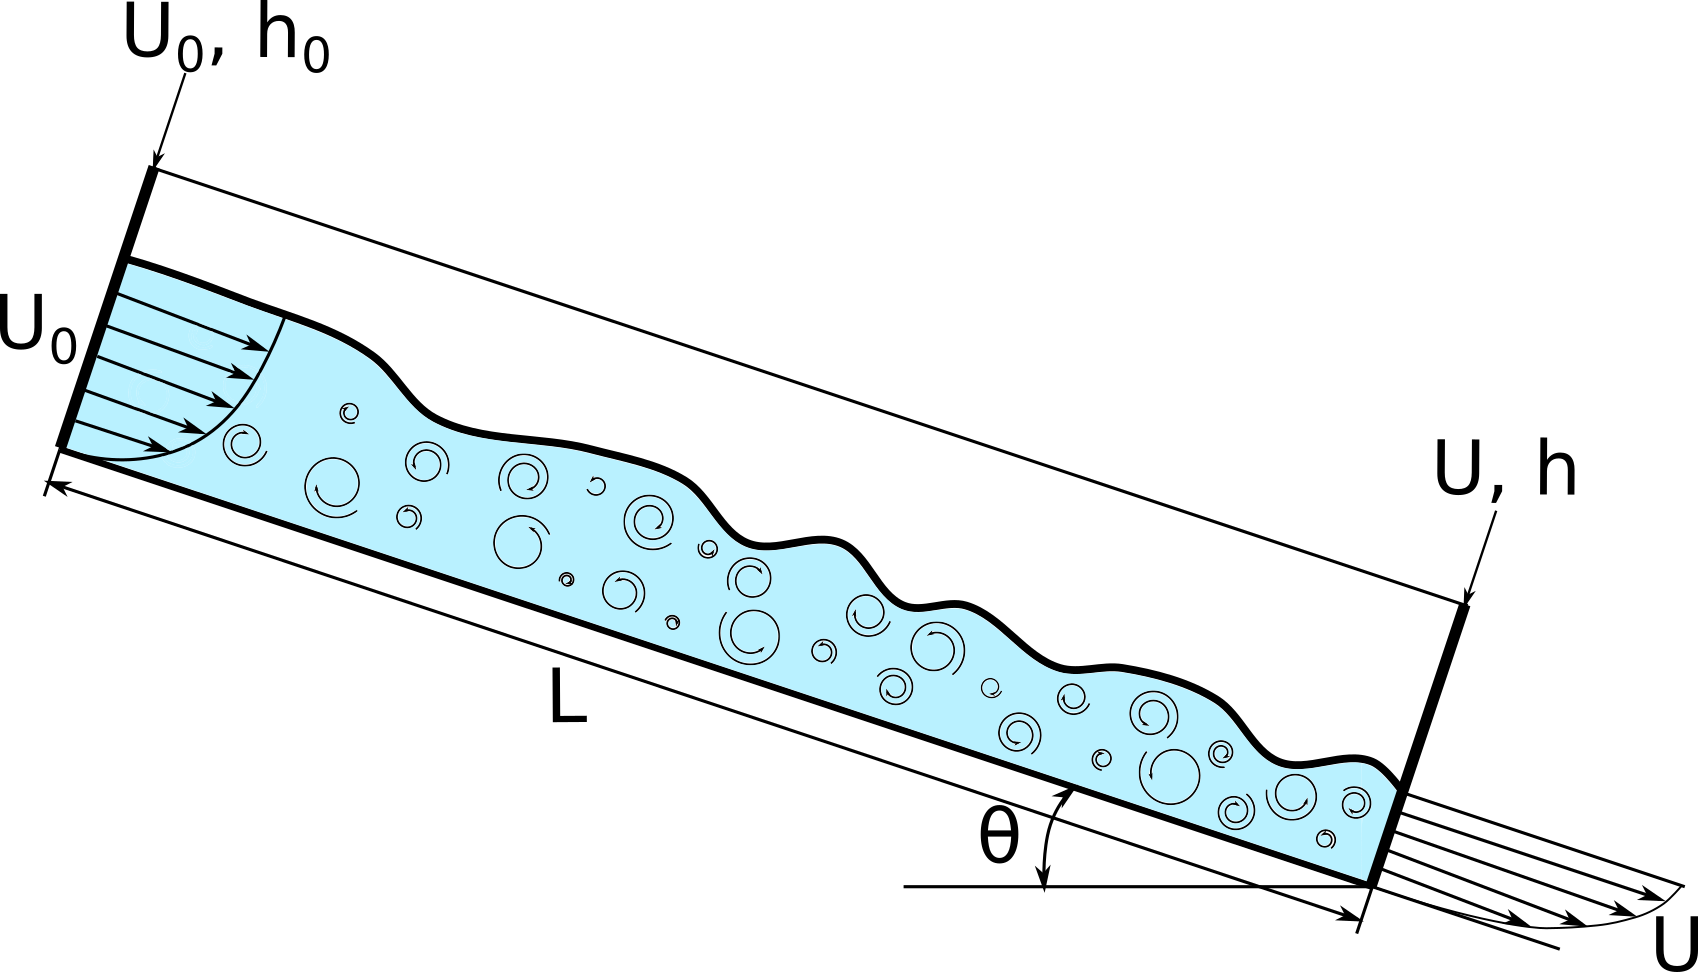
\includegraphics[width=10.5 cm]{NIIMexLinearUProfileInlet.png}
\caption{Принципиальная схема экспериментального желоба.\label{NIIMexLinearUProfileInlet}}
 
\end{figure}   
 

Эксперимент проводился в стационарном режиме. Стационарность обеспечивал погружной насос ``ДЖИЛЕКС Фекальник 200'' производительностью 200 л в минуту. Измерение проводилось с помощью трубки Пито, соединенной с датчиком давления ``КОРУНД-ДДН-001М'' с погрешностью 0,1\%. Точки измерения располагались через каждые 0.5 мм. Для каждого измерения использовалось осреднение значения в течении 10 с. Температура воды в эксперименте составляла 20 градусов Цельсия (комнатная температура). Все коэффициенты модели, связанные с температурой, были выбраны на основе этого значения. 

Было проведено 3 серии экспериментов, в которых менялся угол наклона склона, начальная глубина потока, начальный профиль потока, как показано в таблице~\ref{tabNIIMexLinear}~\cite{fluids7030111}, где $u_0$~--- осреднённая по глубине скорость, $h_0$~--- глубина потока, $\theta$~--- угол наклона склона.

\begin{table}[H] 
\caption{Параметры эксперимента~\cite{fluids7030111}.\label{tabNIIMexLinear}}
\newcolumntype{C}{>{\centering\arraybackslash}X}
\begin{tabularx}{\textwidth}{CCC}
\toprule
    \textbf{$\boldsymbol{u_0}$, м/с}	&    \textbf{$\boldsymbol{h_0}$, мм}	&     \textbf{$\boldsymbol{\theta}$}\\
\midrule
	1.63 & 4.20 & 25$^\circ$\\
	2.00 & 4.95 & 28$^\circ$\\
	1.78 & 3.45 & 33$^\circ$\\
\bottomrule
\end{tabularx}
\end{table}
\unskip

%%%%%%%%%%%%%%%%%%%%%

%ННГУ

\section{Математическая модель}\label{math_model}

Для расчёта эксперимента поставленного в НИИ Механики МГУ используются осреднённые по Рейнольдсу уравнения Навье-Стокса~\cite{Wilcox2006, Hirsch2007,FerzigerPeric2002}. Для получения значений тензора напряжений Рейнольдса используется замыкание в виде $k-\omega\ SST$ модели турбулентности~\cite{Menter1993, Menter1994}. Положение свободной поверхности потока определяется с использованием метода объёма жидкости VOF (Volume Of Fluid), предложенного Хиртом и Николсом в 1981 году~\cite{Hirt1981}. В данном методе используется величина объёмной доли фазы воды $\alpha$ в ячейке для определения свободной поверхности таким образом, что при $\alpha>0.6$ считается что ячейка заполнена жидкостью, в противном случае~--- воздухом.

Течение в экспериментальной у становке описывается системой из пяти уравнений \eqref{vofKWSST}. Это уравнения Навье-Стокса, осреднённые по Рейнольдсу (уравнение неразрывности и уравнение сохранения импульса). Так же в систему входит уравнение переноса объёмной доли фазы для отслеживания межфазной границы. Замыкают систему уравнения сохранения для турбулентной кинетической энергии и специальной диссипации турбулентной кинетической энергии, которые используются для вычисления напряжений Рейнольдса, возникающих при осреднении уравнений Навье-Стокса.
\begin{linenomath} 
%MDPI: Please confirm if bold in equations is necessary. Please check the whole paper
%Authors: Bold is not necessary. Removed
\begin{equation}
	\label{vofKWSST}
	\left\{
		\begin{aligned}
			&{\nabla} \cdot \bar{{u}} = 0,\\
			&\frac{\partial \alpha}{\partial t} + {\nabla} \cdot (\bar{{u}} \alpha) = 0,\\
			&\frac{\partial (\rho \bar{{u}})}{\partial t} + {\nabla} \cdot (\rho \bar{{u}} \bar{{u}}) = -{\nabla} \bar{p} + {\nabla} \cdot \bar{{\tau}} + \rho \bar{{f}},\\
			&\frac{\partial (\rho k)}{\partial t} + {\nabla} \cdot (\rho \bar{{u}} k) = \widetilde{P}_k - \beta^*\rho k \omega + {\nabla} \cdot \left( (\mu + \alpha_k \mu_t) {\nabla} k \right),\\
			&\frac{\partial (\rho \omega)}{\partial t}  + {\nabla} \cdot ( \rho \bar{{u}} \omega) = \gamma \rho \dot{s}^2 - \beta \rho \omega^2 + {\nabla} \cdot \left( (\mu + \alpha_\omega \mu_t) {\nabla} \omega \right) + \\
			&2 (1 - F_1) \rho \alpha_{\omega 2} \frac{1}{\omega} {\nabla} k \cdot {\nabla} \omega.
		\end{aligned}
	\right.
\end{equation}
\end{linenomath}

Здесь ${u}$~--- скорость смеси; $\alpha$~--- объёмная доля выбранной фазы; $\rho$~--- плотность смеси, рассчитываемая по принципу весового среднего; $\bar{ {\tau}} = 2 \mu_{eff} \bar{ {s}}$~--- тензор напряжений, выраженный через тензор скоростей деформации $\bar{ {s}}$, горизонтальной чертой над буквами обозначается осреднение по Рейнольдсу; $\mu_{eff} = \mu + \mu_t$~--- эффективный коэффициент вязкости, сумма молекулярной вязкости и турбулентной, последняя вычисляется по формуле $\mu_t = \rho a_1 k / \max(a_1 \omega,\ b_1 \dot{s} F_2)$; $\bar{p}$~--- давление; $\bar{ {f}}$~--- плотность массовых сил; $k$---плотность турбулентной кинетической энергии; $\omega$---специальная скорость диссипации турбулентной кинетической энергии; $F_1 = \tanh \left( \left( \min\left( \max \left( \frac{\sqrt{k}}{\beta^* \omega y},\ \frac{500 \nu}{y^2 \omega} \right),\ \frac{4 \rho \alpha_{\omega 2} k}{CD_{k \omega} y^2} \right) \right)^4 \right)$~--- функция перемешивания ($F_1$ равняется нулю вдалеке от стены и получается $k-\varepsilon$ модель, и переключается на единицу внутри пограничного слоя, реализуя $k-\omega$ модель); $\dot{s}$~--- скорость сдвига (инвариантная мера $\overline{ {s}}$);  $CD_{k\omega} = \max \left( 2 \rho \alpha_{\omega 2} \frac{1}{\omega}  {\nabla} k \cdot  {\nabla} \omega,\ 10^{-10} \right)$; $F_2 = \tanh \left( \left( \max \left( \frac{2 \sqrt{k}}{\beta^* \omega y},\ \frac{500 \nu}{y^2 \omega} \right) \right)^2 \right)$~--- вторая функция перемешивания, $\widetilde{P}_k = \min (\mu_t  {\nabla} \bar{ {u}} \cdot \left[  {\nabla} \bar{ {u}} + ( {\nabla} \bar{ {u}})^T\right],\ 10 \cdot \beta^* \rho k \omega)$~--- ограничитель на нарастание турбулентности в режимах стагнации. Подробности можно найти в руководстве пользователя пакета OpenFOAM~\cite{OFUG}.
\nomenclature{$u_0$		}{ осредненная по глубине скорость на входной плоскости экспериментального желоба	}
\nomenclature{$h_0$		}{ глубина потока на входной плоскости экспериментального желоба	}
\nomenclature{$\theta$	}{ угол наклона экспериментального желоба }
\nomenclature{$\alpha$	}{ объемная доля воды	}
\nomenclature{$\bar{ {\tau}}$	}{ тензор напряжений осредненный по Рейнольдсу	}
\nomenclature{$\bar{ {s}}$		}{ тензор скоростей деформаций осредненный по Рейнольдсу	}
\nomenclature{$\mu_{eff}$		}{ эффективная вязкость	}
\nomenclature{$\mu$		}{ молекулярная вязкость	}
\nomenclature{$\mu_{t}$		}{ турбулентная вязкость	}
\nomenclature{$\bar{ {f}}$		}{ плотность массовых сил, осреднённая по Рейнольдсу	}
\nomenclature{$\bar{ {u}}$		}{ скорость смеси осреднённаятпо Рейнольдсу	}
\nomenclature{$\rho$		}{ плотность смеси	}
\nomenclature{$\bar{p}$		}{ давление в смеси	}
\nomenclature{$\omega$		}{ специальная скорость диссипации турбулентной кинетической энергии	}
\nomenclature{$k$		}{ 	турбулентная кинетиченская энергия }
\nomenclature{$F_1$		}{ первая функция перемешивания	}
\nomenclature{$\dot{ {s}}$		}{ осредненная по Рейнольдсу скорость деформации	}
\nomenclature{$F_2$		}{ вторая функция перемешивания	}
\nomenclature{$\widetilde{P}_k$ }{ ограничитель нарастания турбулентности, используемый в режимах стагнации }

Турбулентная модель содержит четыре коэффициента: $\alpha_k$, $\alpha_\omega$, $\beta$, $\gamma$. $\alpha_k$, $\alpha_\omega$, $\gamma$ рассчитываются по принципу весового среднего: $\gamma = \gamma_1 F_1 + \gamma_2 (1 - F_1)$. Стандартно константы турбулентной модели задаются следующими значениями~\cite{LaunderSpalding1974, Tahry1983, LaunderMorseRodiSpaldiug1972}:
\begin{linenomath}
\begin{equation}
	\label{kOmegaSstConstantsInit}
	\begin{aligned}
		\gamma_1 = 5 / 9,\ \ \ \beta_1 = 3 / 40,\ \ \ \alpha_{k1} = 0.85,\ \ \ \alpha_{\omega1} = 0.5,\\
		\gamma_2 = 0.44,\ \ \ \beta_2 = 0.083,\ \ \ \alpha_{k2} = 1,\ \ \ \alpha_{\omega 2} = 0.856,\\
		\beta^* = 0.09,\ \ \ a_1 = 0.31,\ \ \ b_1 = 1.0,\ \ \ c_1 = 10.0.
	\end{aligned}
\end{equation}
\end{linenomath}

\nomenclature{$\alpha_k$ }{ коэффициент замыкания модели турбулентности }
\nomenclature{$\alpha_{k1}$ }{ коэффициент замыкания модели турбулентности }
\nomenclature{$\alpha_{k2}$ }{ коэффициент замыкания модели турбулентности }
\nomenclature{$\alpha_\omega$ }{ коэффициент замыкания модели турбулентности }
\nomenclature{$\alpha_{\omega1}$ }{ коэффициент замыкания модели турбулентности }
\nomenclature{$\alpha_{\omega2}$ }{ коэффициент замыкания модели турбулентности }
\nomenclature{$\beta$ }{ коэффициент замыкания модели турбулентности }
\nomenclature{$\beta_1$ }{ коэффициент замыкания модели турбулентности }
\nomenclature{$\beta_2$ }{ коэффициент замыкания модели турбулентности }
\nomenclature{$\gamma$ }{ коэффициент замыкания модели турбулентности }
\nomenclature{$\gamma_1$ }{ коэффициент замыкания модели турбулентности }
\nomenclature{$\gamma_2$ }{ коэффициент замыкания модели турбулентности }
\nomenclature{$\beta^*$ }{ коэффициент замыкания модели турбулентности }
\nomenclature{$a_1$ }{ коэффициент замыкания модели турбулентности }
\nomenclature{$b_1$ }{ коэффициент замыкания модели турбулентности }
\nomenclature{$c_1$ }{ коэффициент замыкания модели турбулентности }

Детали описания модели турбулентности представлены в~\cite{Menter1993, MenterKuntzLangtry2003}.
 
%%%%%%%%%%%%%%%%%%%%%%%%%%%%%%%%%%%%%%%%%%
\section{Методы}\label{sec4}
%ИСП
%\subsection{Используемый численный метод решения ДУЧП}
\subsection{Вычислительные методы гидродинамики}

Для реализации трехмерного многофазного односкоростного подхода использовался решатель interFoam~\cite{Rusche2003ComputationalFD} пакета OpenFOAM (v2012, созданный Генри Веллером в 1989 г., Бракнелл, Великобритания).

Используются следующие аппроксимационные схемы:
\begin{itemize}
	\item производные по времени $\frac{\partial}{\partial t}$ аппроксимируются с помощью неявного метода Эйлера;
	\item поток объёмной доли фазы $ {\nabla} \cdot (\bar{ {u}} \alpha)$ аппроксимируется при помощи схемы Ван Лира;
	\item поток массы смеси $ {\nabla} \cdot (\rho \bar{ {u}} \bar{ {u}})$ аппроксимируется с помощью противопоточной схемы с весами;
	\item дивергенция тензора вязких напряжений $ {\nabla} \cdot \bar{ {\tau}}$ аппроксимируется с помощью центральной разностной схемы;
	\item поток турбулентной кинетической энергии $ {\nabla} \cdot (\rho \bar{ {u}} k)$ аппроксимируется противопоточной схемой;
	\item поток специальной диссипации турбулентной кинетической энергии $ {\nabla} \cdot (\rho \bar{ {u}} \omega)$ используется противопоточная схема;
	\item оператор градиента $ {\nabla}$ аппроксимируется центрально-разностной схемой;
	\item оператор Лапласа $ {\nabla}^2$ аппроксимируется центрально-разностной схемой с явной неортогональной коррекцией;
	\item другие, не перечисленные выше члены описываются с помощью центрально-разностной схемы.
\end{itemize}

Линейная противопоточная схема второго порядка, используемая для конвекционного члена, является наиболее эффективной и точной для моделирования усредненного Рейнольдса Навье--Стокса (RANS)~\cite{ROBERTSON2015122}.

Алгоритм PIMPLE~\cite{Holzmann2019, Yin2003}, который был разработан для решения уравнений с большим числом Куранта, использовался для решения системны уравнений. PIMPLE представляет собой комбинацию алгоритмов PISO~\cite{Issa1986_2} и SIMPLE~\cite{Issa1986_1}.

% To solve the system of equations, the PIMPLE~\cite{Holzmann2019, Yin2003} algorithm was used. This algorithm is a combination of the PISO (Pressure Implicit with Splitting of Operator)~\cite{Issa1986_2} and the SIMPLE (Semi-Implicit Method for Pressure-Linked Equations) algorithms~\cite{Issa1986_1}.
%

Метод сопряженных градиентов с предобуславливателем GAMG используется для решения системы линейных уравнений для давления. В качестве сглаживателя используется метод Гаусса-Зейделя. Значения объемной доли воды, скорости, $k$, $\omega$ вычисляются с помощью smoothSolver и метода symGaussSeidel для сглаживания.

\subsubsection{Расчётная область}

Преимущество математического моделирования состоит в том, что модель позволяет размещать виртуальные датчики в любой точке расчетной области для измерения значений физических величин. В эксперименте физические датчики располагались на выходе из желоба. Для сравнения результатов эксперимента и расчета виртуальные датчики располагались в одном и том же месте.

Моделировался участок экспериментального желоба, расположенный между двумя точками измерения профиля скорости и глубины потока.
Моделирование проводилось для 10-мм среза части желоба, где влияние боковых стенок было небольшим.
Первый измеренный профиль использовался в качестве входных данных для расчетной области. Второй был объектом сравнения. 
%
В качестве числовой области использовался параллелепипед размером 590 мм в длину, 10 мм в ширину и 10 мм в высоту.
%
Мы проверили влияние разрешения сетки. Сходимость по сетке изучалась для различных размеров сетки: $290 \times 10 \times 30$, $590 \times 10 \times 60$, $1080 \times 10 \times 120$, и $2160 \times 10 \times 240$. Для каждого прогона профиль выходной скорости сравнивался с экспериментальным с использованием функции потерь \eqref{LossFunction}. Значения функций потерь для трех последних размеров сетки варьировались в пределах 0.1\%. Поэтому количество ячеек было выбрано равным $590 \times 10 \times 60$ из соображений сокращения машинного времени при сохранении точности.

\subsubsection{Начальные и граниченые условия}

Были выделены следующие границы расчётной области: дно лотка, боковые стенки лотка, верхняя граница лотка, плоскость на входе в лоток, плоскость на выходе из лотка.

Были заданы следующие граничные условия:
\begin{itemize}
	\item Дно лотка является твёрдой стенкой с условием прилипания потока; 
	\item На боковых стенках лотка задано условие нулевого градиента для реализации отсутствия влияния стенок на поток;
	\item Для верхней границы расчетной области использовалось смешанное условие с атмосферным давлением, отсутствием притока через границу и оттоком по условию нулевого градиента, задано условию фиксированного значения для $k$ и $\omega$;
	\item Для входной плоскости использовались фиксированные значения объемной доли воды, профиля скорости, значений $k$ и $\omega$;
	\item Для выходной плоскости использовалось условие нулевого градиента.
\end{itemize}

Математическая формулировка перечисленных начальных и граничных условий представлена в руководстве пользователя OpenFOAM~\cite{OFUG}.

Среднее значение $Y+$ равно 17, что допускает использование модели пристеночных функций. Функция nutkWallFunction использовалась в качестве граничного условия для стенки, которая обеспечивает ограничение турбулентной вязкости стенкой на основе турбулентной кинетической энергии для моделей турбулентности как с низким, так и с высоким числом Рейнольдса.

Начальные условия в задаче задаются так, чтобы объем был полностью заполнен неподвижным воздухом, а жидкость втекала через входную плоскость. Через некоторое время поток устанавливается и проводятся измерения на выходной плоскости для сравнения с экспериментальными данными. Шаг по времени $dt$ равен 0,001 с. Поток считается установившимся через 5 с.


%%%%%%%%%%%%%%%%%%%%Перенести в раздел с оптимизацией


%При оптимизации коэффициентов турбулентной модели минимизируется корень из среднеквадратического отклонения вычисленного профиля скорости потока на выходной плоскости от экспериментального профиля:



%%%%%%%%%%%%%%%%%%%%%%%%%%%%%%%%%%%%%%%%%%


%Для расчёта эксперимента НИИ Механики МГУ была рассчитана часть экспериментального лотка, находящаяся между двумя точками замера профиля скорости и глубины потока. Расчёт проводился для срединной полоски лотка толщиной 10~мм, где влияние боковых стенок незначительно. Первый измеренный профиль подавался на вход расчётной области, второй являлся объектом сравнения. Геометрия расчётной области представляет собой параллелепипед длинной 590~мм, шириной 40~мм, и глубиной 10~мм. Количество ячеек составило 590х10х60.



%Более детальное описание математической модели можно найти в книге Ферцигера и Перича~\cite{FerzigerPeric2002}.



%ННГУ
\subsection{Постановка задачи глобальной оптимизации}
Программное обеспечение Globalizer (ННГУ им. Н.И. Лобачевского) использовалось для решения оптимизационный задачи.
Будем предполагать, что выбор того или иного набора значений параметров модели определяется значениями вектора $y=(y_1,y_2,...,y_N)$, а качество модели, соответствующие заданному значению вектора параметров, описывается функцией $\varphi(y)$. Будем называть данную функцию критерием оптимизации, причем уменьшение значения критерия соответствует более хорошей математической модели. Также будем предполагать, что должны выполняться некоторые требования, гарантирующие применимость модели. Выполнение указанных требований обычно формулируется как условие принадлежности вектора $y$ гиперинтервалу $D$,
\begin{linenomath}
\begin{equation}
D=\{a_i \leq y_i \leq b_i, \; 1 \leq i \leq N\}.
\end{equation}
\end{linenomath}
\nomenclature{$y = (y_1, ..., y_N)$ }{ вектор параметров}
\nomenclature{$\varphi(y)$ }{целевая функция }
\nomenclature{$D$ }{гиперинтервал}

Таким образом, процессу выбора оптимального набора параметров модели соответствует задача глобальной оптимизации вида:
\begin{linenomath}
\begin{equation}\label{main_problem}
\begin{aligned}
    & \varphi(y^\ast)=\min{\left\{\varphi(y):y\in D\right\}},\\
    & D=\left\{y\in \text{R}^N: a_i\leq y_i \leq b_i, 1\leq i \leq N\right\}.
\end{aligned}
\end{equation}
\end{linenomath}
При оптимизации коэффициентов турбулентной модели учитывается среднеквадратическая ошибка дифференцирования расчетного профиля скорости потока и экспериментального на выходной плоскости 
%MDPI: Please confirm if bold in equations is necessary. Please check the whole paper
%Authors: Bold is not necessary. Removed
\begin{linenomath}
\begin{equation}
	\label{LossFunction}
	 {L_{RMSE}} = \sqrt{\frac{\sum\limits_{i=1}^{N} \left( u_{EXP}^i - u_{k-\omega\ SST}^i \right)^2}{N}}.
\end{equation}
\end{linenomath}

Здесь $u_{EXP}^i$ — горизонтальная составляющая скорости в контрольной точке, полученная опытным путем, а $u_{k-\omega\ SST}^i$ — горизонтальная составляющая скорости в контрольной точке, рассчитанная по формуле гидродинамики, $N$ - количество точек сравнения горизонтальной составляющей скорости по глубине потока в выходной плоскости (правое сечение показано на рисунке \ref{NIIMexLinearUProfileInlet}). Используется примерно 10 точек сравнения. Их количество определяется количеством измерений, выполненных в эксперименте, и варьируется в зависимости от изменения глубины потока при различных углах наклона желоба. Точки равномерно распределены по глубине для работы средств измерения, используемых в эксперименте.

\nomenclature{$N$ }{ количество точек измерения скорости по глубине потока в выходной плоскости }
\nomenclature{$u^i_{EXP}$ }{ горизонтальная составляющая скорости в контрольной точке, полученная экспериментальным путем }
\nomenclature{$u^i_{k-\omega}\ SST$ }{ горизонтальная составляющая скорости в контрольной точке, рассчитанная методом CFD }
\nomenclature{$ {L_{RMSE}}$ }{ функция потерь }

Будем рассматривать функцию потерь (\ref{LossFunction}) как целевую функцию $\varphi(y)$ в задаче глобальной оптимизации (\ref{main_problem}). Рассматриваемые задачи характеризуются тем фактом, что целевая функция $\varphi(y)$ не задана аналитически; есть лишь некоторый алгоритм вычисления ее значений в точках области $D$. При этом одно поисковое испытание соответствует одному расчету по модели и является вычислительно-трудоемкой операцией \cite{Kalyulin2017,Paulavicius2020}.

Задачи многоэкстремальной оптимизации имеют существенно более высокую трудоемкость решения по сравнению с другими типами оптимизационных задач, т.к. глобальный оптимум является интегральной характеристикой решаемой задачи и требует исследования всей области поиска. Как результат, поиск глобального оптимума сводится к построению некоторого покрытия (сетки) в области параметров, и выборе наилучшего значения функции на данной сетке. Снижение объема вычислений может быть достигнуто при построении неравномерного покрытия области поиска: сетка должна быть достаточно плотной в окрестности глобального оптимума и более редкой вдали от искомого решения.

Типичным предположением, которое используют многие методы глобальной оптимизации \cite{Sergeyev2013,Evtushenko2013,Jones2009,Zilinskas2010}, является предположение о том, что целевая функция $\varphi(y)$ удовлетворяет условию Липшица
\begin{linenomath}
\begin{equation}
\left|\varphi(y_1)-\varphi(y_2)\right|\leq L\left\|y_1-y_2\right\|,\; y_1,y_2 \in D, \; 0<L<\infty,
\end{equation}
\end{linenomath}

Предположение такого рода является достаточно естественным для многих прикладных задач, поскольку относительные изменения функции, характеризующей моделируемый процесс, обычно не могут превышать некоторый порог, определяемый ограниченной энергией изменений. Возникающий при этом вопрос об оценке априори неизвестных значений константы Липшица может решаться путем введения адаптивных схем \cite{Strongin2020,Strongin2020_1}.
\nomenclature{$L$		}{ константа Липшица	}

Существует несколько способов адаптации эффективных одномерных алгоритмов для решения многомерных задач (см., например,~\cite{Sergeyev2017,Zilinskas2014}). В этом исследовании мы применяем уменьшение размерности с помощью кривой Пеано $y(x)$, непрерывно отображающей единичный интервал [0,1] на $n$-мерный куб
\begin{linenomath}
\begin{equation}
\left\{y\in R^N: -2^{-1}\leq y_i \leq 2^{-1}, 1 \leq i \leq N\right\}=\left\{y(x):0\leq x \leq 1 \right\}.
\end{equation}
\end{linenomath}

Алгоритмы построения кривых заполнения пространства типа Пеано и соответствующая теория подробно рассмотрены в~\cite{Strongin2000,Sergeyev2013}.

С помощью такого отображения многомерная задача~(\ref{main_problem}) может быть сведена к одномерной задаче вида
\begin{linenomath}
\begin{equation}
\varphi(y^\ast)=\varphi(y(x^\ast))=\min{\left\{\varphi(y(x)): x\in[0,1]\right\}}.
\end{equation}
\end{linenomath}

Важным свойством такого отображения является то, что если функция $\varphi(y)$ в области $D$ удовлетворяет условию Липшица, то функция $\varphi(y(x))$ на интервале $[0,1 ]$ будет удовлетворять равномерному условию Гёльдера
\begin{linenomath}
\begin{equation}
\left|\varphi(y(x_1))-\varphi(y(x_2))\right|\leq H\left|x_1-x_2\right|^{1/N},
\end{equation}
\end{linenomath}
где константа Гельдера $H$ связана с константой Липшица $L$ соотношением $H=2L\sqrt{N+3}$~\cite{Strongin2000}.
\nomenclature{$H$		}{ константа Гёльдера	}


Следовательно, мы можем рассмотреть минимизацию одномерной функции
\begin{linenomath}
\begin{equation}
f(x)=\varphi(y(x)), \;\; x\in[0,1],
\end{equation}
\end{linenomath}
удовлетворяющее условию Гёльдера.
\nomenclature{$y(x)$		}{ кривая Пеано	}
\nomenclature{$f(x) = \varphi(y(x))$		}{ одномерная функция	}


%\newpage


\subsection{Алгоритм Глобального Поиска}\label{GSA}

Алгоритм решения задачи (\ref{main_problem}) заключается в построении последовательности точек $x^k$, в которых вычисляются значения целевой функции $z^k = f(x^k)=\varphi(y(x ^k))$. Назовем процесс вычисления значения функции (включая построение изображения $y^k=y(x^k)$) "испытанием", а пару $(y^k, z^k) $, "результатом испытания". Набор пар $\left\{(y^k, z^k), 0\leq k\leq n\right\}$ составляет поисковую информацию, собранную методом после выполнения $n$ шагов. Правила, определяющие работу \textit{алгоритма глобального поиска}, следующие.

Первые два испытания выполняются в граничных точках отрезка $[0,1]$, т.е. $x^0 = 0$ и $x^1 = 1$. Вычисляются значения целевой функции $z^0 = f(x^0)$ и $z^1 = f(x^1)$ и устанавливается счетчик $k = 1$. Очередная точка испытания $x^{k+1}, k \geq 1,$ выбирается по следующим правилам.

Шаг 1. Перенумеровать точки множества $X_k=\{x^0,\dots,x^k\}$ нижними индексами в порядке возрастания значений координат, т.е.
\begin{linenomath}
\begin{equation}
0=x_0<x_1<\dots <x_{k-1}<x_{k}=1.
\end{equation}
\end{linenomath}
\nomenclature{$X_k=\{x^0,\dots,x^k\} $ }{ набор точек испытаний }
Обратите внимание, что здесь и далее верхние индексы используются для обозначения номера итерации, а нижние индексы — для нумерации точек по порядку.

Шаг 2. Предположим, что $z_i=f(x_i), \; 1\leq i \leq k$. Рассчитать значения
\begin{linenomath}
\begin{equation}\label{mu}
\mu = \max_{1\leq i \leq k}\frac{\left|z_i-z_{i-1}\right|}{\Delta_i},
\end{equation}
\end{linenomath}
\begin{linenomath}
\begin{equation}
M = \left\{
   \begin{array}{lr}
     r\mu, & \mu > 0,\\
     1, & \mu = 0,
   \end{array}
\right.
\end{equation}
\end{linenomath}
где действительное число $r>1$ — входной параметр метода, а $\Delta_i=\left(x_i-x_{i-1}\right)^{1/N}$.

\nomenclature{$z^k = f(x^k)$ }{ значение целевой функции }
\nomenclature{$M$ }{ адаптивная оценка константы Липшица }
\nomenclature{$r>0$ }{ параметр метода }

Шаг 3. Для каждого интервала $(x_{i-1}, x_i), \; 1\leq i \leq k,$ рассчитать характеристику по следующей формуле
\begin{equation}\label{R}
R(i)=\Delta_i+\frac{(z_i-z_{i-1})^2}{M^2\Delta_i}-2\frac{z_i+z_{i-1}}{M},1 \leq i \leq k.
\end{equation}

\nomenclature{$R(i)$ }{ характеристика $i$-го интервала поиска}

Шаг 4. Выбрать интервал $(x_{t-1},x_t)$, соответствующий максимальной характеристике
\begin{equation}\label{MaxR}
R(t)=\max{\left\{R(i): 1 \leq i \leq k \right\}}.
\end{equation}

Шаг 5. Выполнить новое испытание в точке $x^{k+1}\in(x_{t-1},x_t)$, рассчитанной по следующей формуле
\begin{equation}\label{NewX}
x^{k+1} = \frac{x_t+x_{t-1}}{2} - \mathrm{sign}(z_t-z_{t-1})\frac{1}{2r}\left[\frac{\left|z_t-z_{t-1}\right|}{\mu}\right]^N.
\end{equation}

Алгоритм останавливается, когда $\Delta_t<\epsilon$, где $\epsilon>0$ — заданная точность. Для оценки значения глобального оптимума использовать формулу
\begin{linenomath}
\begin{equation}
f_k^\ast=\min_{0\leq i \leq k}f(x^i), \ x_k^\ast=\arg \min_{0\leq i \leq k}f(x^i),
\end{equation}
\end{linenomath}

Строгое доказательство сходимости этого алгоритма приведено в~\cite{Strongin2000}.
%The modifications taking into account existence of inequality constraints in the problem and the information about the objective function derivative are given in~\cite{RefBarkalov,RefGergel1996,RefGergel1997}

%\newpage

\subsection{Построение аппроксимации целевой функции}

\subsubsection{Использование нейронных сетей}

Не существует универсальных правил выбора топологии нейронной сети для решения конкретной задачи. Однако в~\cite{Cybenko1989} теорема Колмогорова была обобщена и доказано, что любая непрерывная функция от $N$ переменных может быть аппроксимирована трехслойной искусственной нейронной сетью прямого распространения с одним скрытым слоем и алгоритмом обратного распространения ошибки в виде обучающий с любой степенью точности. Эта теорема называется теоремой универсального приближения или теоремой Цыбенко~\cite{Hassoun1995}.

Универсальных правил выбора топологии нейронной сети для решения той или иной задачи не существует. Однако в~\cite{Cybenko1989} была обобщена теорема Колмогорова и было доказано, что любая непрерывная функция $N$ переменных может быть аппроксимирована трехслойной искусственной нейронной сетью прямой связи с одним скрытым слоем и алгоритмом обратного распространения ошибки в качестве обучающего алгоритма с любой степенью точности. Данная теорема носит название \textit{Универсальная теорема аппроксимации} или теорема Цыбенко \cite{Hassoun1995}.

Нейронные сети в качестве аппроксиматора реализованы во многих библиотеках машинного обучения. 
В проведенном исследовании для построения аппроксимации целевой функции был использован класс MLPRegressor из библиотеки машинного обучения Scikit-learn. Он реализует многослойный персептрон (MLP), который обучается с использованием обратного распространения ошибки без функции активации в выходном слое~\cite{Nielsen1989}. MLP продемонстрировали способность находить приближенные решения для чрезвычайно сложных задач.
На Figure \ref{fig1} показан MLP с одним скрытым слоем со скалярным выходом

\begin{figure}[H]
 
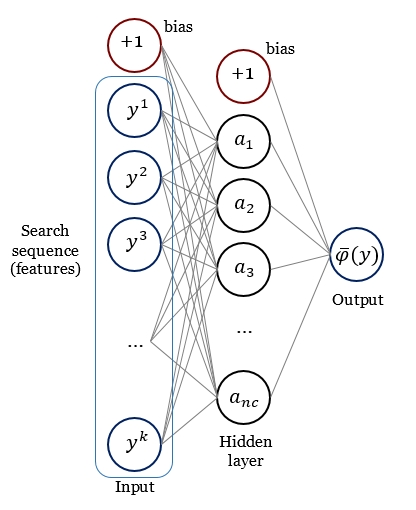
\includegraphics[width=5 cm]{perceptron.jpg}
\caption{Трехслойный перцептрон со скалярным выходом.\label{fig1}}
 
\end{figure}

Левый слой, называемый входным, состоит из набора нейронов $y_i, \; i=\overline{1,k}$, представляющих входные сигналы (значения переменных). Каждый нейрон скрытого слоя преобразует значения из предыдущего слоя взвешенным линейным суммированием.
\begin{linenomath}
\begin{equation}
w_1 y_1 + w_2 y_2+...+w_k y_k+bias,
\end{equation}
\end{linenomath}
где $w_i$ — веса нейронов, а $bias$ — специальный вес, который не имеет множителя в виде входного значения. Далее полученное значение преобразуется в выходное (прогнозируемое) значение слоя с помощью передаточной функции (функции активации). Выходной слой получает значения из последнего скрытого слоя и преобразует их в выходные значения. Обучение сети осуществляется методом обратного распространения ошибки.

Мы использовали трехслойную нейронную сеть для решения задачи аппроксимации по следующим причинам. С теоретической точки зрения такой сети будет достаточно для аппроксимации функции с высокой точностью. С практической точки зрения использование глубоких нейронных сетей здесь будет избыточным, так как набор результатов испытаний, используемых для построения аппроксимации, невелик и не будет достаточным для обучения глубокой сети.

\subsubsection{Выбор параметров модели}

Выбор решателя, функция активации, значение параметра регуляризации, количество нейронов в скрытом слое и т. д. являются переменными параметрами настройки нейронной сети.
Например, для небольших наборов многомерных данных лучше и быстрее демонстрирует себя решатель lbfgs, являющийся модификацией алгоритма Бройдена--Флетчера--Гольдфарба--Шанно~\cite{Nocedal2006} и относящийся к квазиньютоновским методам. Все численные эксперименты проводились по этому алгоритму.
В качестве функций активации нейронов использовались сигмоидальные функции (логистическая функция или гиперболический тангенс).
Количество нейронов в каждом слое и параметр регуляризации (alpha) подбирались в экспериментах и зависели от конкретной задачи.

В проведенных экспериментах мы выбрали следующую архитектуру сети:

\begin{verbatim}
    model = MLPRegressor(activation='logistic',
	solver='lbfgs',
	alpha=0.001,
	hidden_layer_sizes=(20,),
	max_iter=5000,
	tol=10e-6,
	random_state=10)
\end{verbatim}


\subsection{Использование аппроксимаций при решении задачи оптимизации}\label{GSA_Appr}

В настоящей работе мы применили следующий метод использования аппроксимации целевой функции в задачах оптимизации: по накопленной поисковой информации построить аппроксимацию целевой функции, найти минимум аппроксимации и повторить этот процесс либо до исчерпания вычислительного ресурса, либо до тех пор, пока не будет достигнута сходимость.

Предлагаемый метод будет иметь смысл либо в том случае, когда объем накопленной поисковой информации достаточно велик (что позволяет построить относительно точную аппроксимацию многоэкстремальной функции), либо в случае, когда задача подобна задаче на поиск локального экстремума.
Первый случай соответствует заключительной фазе поиска и может быть интерпретирован как метод уточнения текущего решения. Однако если целевая функция является вычислительно-трудоемкой, невозможно провести достаточно большое количество испытаний. Здесь мы столкнемся с исчерпанием вычислительных ресурсов.

Второй случай предполагает построение хорошей аппроксимации на основе относительно небольшого числа испытаний и, по сути, включает предположение о слабой многоэкстремальности целевой функции, что хорошо согласуется с задачей, рассматриваемой в рамках настоящего исследования.

Алгоритм глобального поиска с использованием аппроксимации целевой функции можно сформулировать следующим образом.
Предположим, что имеющиеся ресурсы позволяют выполнить $K_{max} = K_1 + K_2$ испытаний.

На первом этапе выполняются $k = K_1$ испытаний с использованием базового алгоритма глобального поиска из раздела \ref{GSA}.
Во время выполнения первого этапа происходит накопление множества результатов испытаний $\Omega = \left\{(y^k, \varphi(y^k)), 0\leq k\leq K_1\right\}$, необходимого для построения аппроксимации функции.

На втором этапе алгоритм работает с использованием аппроксимации. Для вычисления точки $y^{k+1}$ очередного $(k+1)$-го испытания выполняются следующие действия.

%Описание работы алгоритма
Шаг 1. По набору результатов испытаний $\Omega$, сформированному в ходе выполнения алгоритма, построить аппроксимацию целевой функции $\overline{\varphi}(y)$;

Шаг 2. Используя базовый алгоритм глобального поиска из раздела \ref{GSA}, найти глобальный минимум функции $\overline{\varphi}(y)$ и использовать это значение в качестве следующей точки испытания, т. е. $y ^{k+1} = \arg \min_{y \in D} \overline{\varphi}(y)$;

Шаг 3.Если выполнено условие $k>K_{max}$, или же выполнено условие $\left\|y^k - y^{k+1}\right\| \leq \epsilon$,  то завершить работу алгоритма.
Иначе выполнить испытание в точке $y^{k+1}$, сохранить его результат в множестве $\Omega$, увеличить счетчик испытаний $k = k+1$ и перейти к шагу 1.

\nomenclature{$\epsilon > 0$ }{ точность поиска }
\nomenclature{$\Omega $ }{ набор результатов испытаний }
\nomenclature{$\overline{\varphi}(y)$}{аппроксимация целевой функции}

Предложенный алгоритм обеспечивает сходимость к глобальному решению в том случае, если выполненных на первом этапе $K_1$ испытаний достаточно для построения аппроксимации целевой функции, адекватно отражающей основные особенности ее поведения.


%пример работы алгоирмта на тестовой задаче?

%%%%%%%%%%%%%%%%%%%%%%%%%%%%%%%%%%%%%%%%%%

%\subsection{Loss function definition}

%%%%%%%%%%%%%%%%%%%%%%%%%%%%%%%%%%%%%%%%%%
\section{Результаты}\label{sec5}

%Описание оборудования и программного обеспечения, которое было задействовано при проведении экспериментов.

%Результаты расчетов

%Иллюстрации

%Сравнение нескольких разных решений (это можно перенести и в следующую секцию)

Вычислительные эксперименты проводились на вычислительном кластере ННГУ им. Н.И. Лобачевского (работает под управлением операционной системы CentOS 7.2). Узел кластера располагает 2-я процессорами Intel Sandy Bridge E5-2660 2.2 GHz, 64 Gb RAM. Центральный процессор является 8-ми ядерным. Рассмотренные в данной работе методы глобальной оптимизации были реализованы на языке C++, использовался компилятор GCC 5.5.0 и openMPI 4.1.1, для построения аппроксимации целевой функции с помощью нейросети использовалась библиотека машинного обучения Scikit-learn из Python 3.9. Для численного решения задачи, описанной в разделе \ref{math_model}, использовалась программа CFD с открытым исходным кодом OpenFOAM v2012~\cite{OpenFOAM}.

%В процессе оптимизации исследовались такие константы, как $\beta^*$, $a_1$, $\alpha_{k 1,2}$, $\alpha_{\omega 1,2}$, которые регулируют скорость диссипации турбулентной кинетической энергии, напряжения Рейнольдса, поток диффузии турбулентной кинетической энергии, поток диффузии диссипации турбулентной кинетической энергии, соответственно.

Перед началом калибровки было проведено небольшое исследование значимости каждого из 12 коэффициентов турбулентной модели. В результате были выявлены несколько наиболее существенных параметров. Было принято решение откалибровать эти коэффициенты. Эти коэффициенты определяют скорость диссипации турбулентной кинетической энергии, напряжение Рейнольдса, диффузионные потоки турбулентной кинетической энергии и удельную скорость диссипации. Коэффициент $\beta^*$ используется в функциях смешивания, описывающих механизм переключения между $k-\varepsilon$ и $k-\omega$. Коэффициент $a_1$ определяет турбулентную вязкость. $\alpha_{k 1,2}$ характеризует поток диффузии турбулентной кинетической энергии. $\alpha_{\omega 1,2}$ характеризуют поток диффузии диссипации турбулентной кинетической энергии.

%Начальные значения коэффициентов были заданы следующими:
Начальные значения коэффициентов
\begin{linenomath}
\begin{equation}
	\begin{aligned}
		\beta^* = 0.09;\ \ \ a_1 = 0.31;\ \ \ \alpha_{k 1} = 0.85;\ \ \ \alpha_{\omega 1} = 0.5; \ \ \ \alpha_{k 2} = 1.0;\ \ \ \alpha_{\omega 2} = 0.856.
	\end{aligned}
\end{equation}
\end{linenomath}

Один расчет целевой функции при заданных значениях параметров занимал в среднем 15 минут с использованием 8 MPI-процессов на узле. 
Подбор оптимальных значений параметров проводился парами, при этом значения остальных параметров -- фиксировались. 
Сначала была выбрана пара наиболее важных параметров $\beta^*$ и $a_1$.
Для исследования поставленной оптимизационной задачи применялись оба возможных подхода к ее решению: без использования аппроксимации целевой функции и с использованием аппроксимации.

В первом эксперименте алгоритм глобального поиска, описанный в разделе \ref{GSA}, применялся без использования аппроксимации.
Параметры метода задавались следующими: $r = 3$ и $\epsilon = 10^{-3}$.
За сутки выполнено 100 итераций алгоритма; требуемая точность не была достигнута.

Во втором эксперименте для решения той же задачи был применен подход, описанный в разделе \ref{GSA_Appr}.
Сначала было выполнено $K_1 = 30$ итераций алгоритма глобального поиска.
После этого был запущен алгоритм, использующий аппроксимацию нейронной сетью.
Всего было выполнено $K_1 + K_2 = 65$ итераций алгоритма, после чего алгоритм остановился на точности.
В результате было найдено наилучшее значение целевой функции 0,375.
Общее время поиска сократилось до 16 ч, что обеспечило более точное решение задачи за разумное время.

Точки испытаний и аппроксимирующая функция, построенная по этим точкам с помощью нейронной сети, представлены на рис.~\ref{NN_100_point} (параметры $\beta^*$ и $a_1$ варьировались). Отчетливо видны несколько локальных минимумов.
Наш анализ показал хорошее соответствие между регрессионной моделью и экспериментальными данными.
Оценка $R^2$ и среднеквадратичное отклонение между прогнозами модели и результатами моделирования равны 0,976 и 0,098 соответственно.


\begin{figure}[H]
 
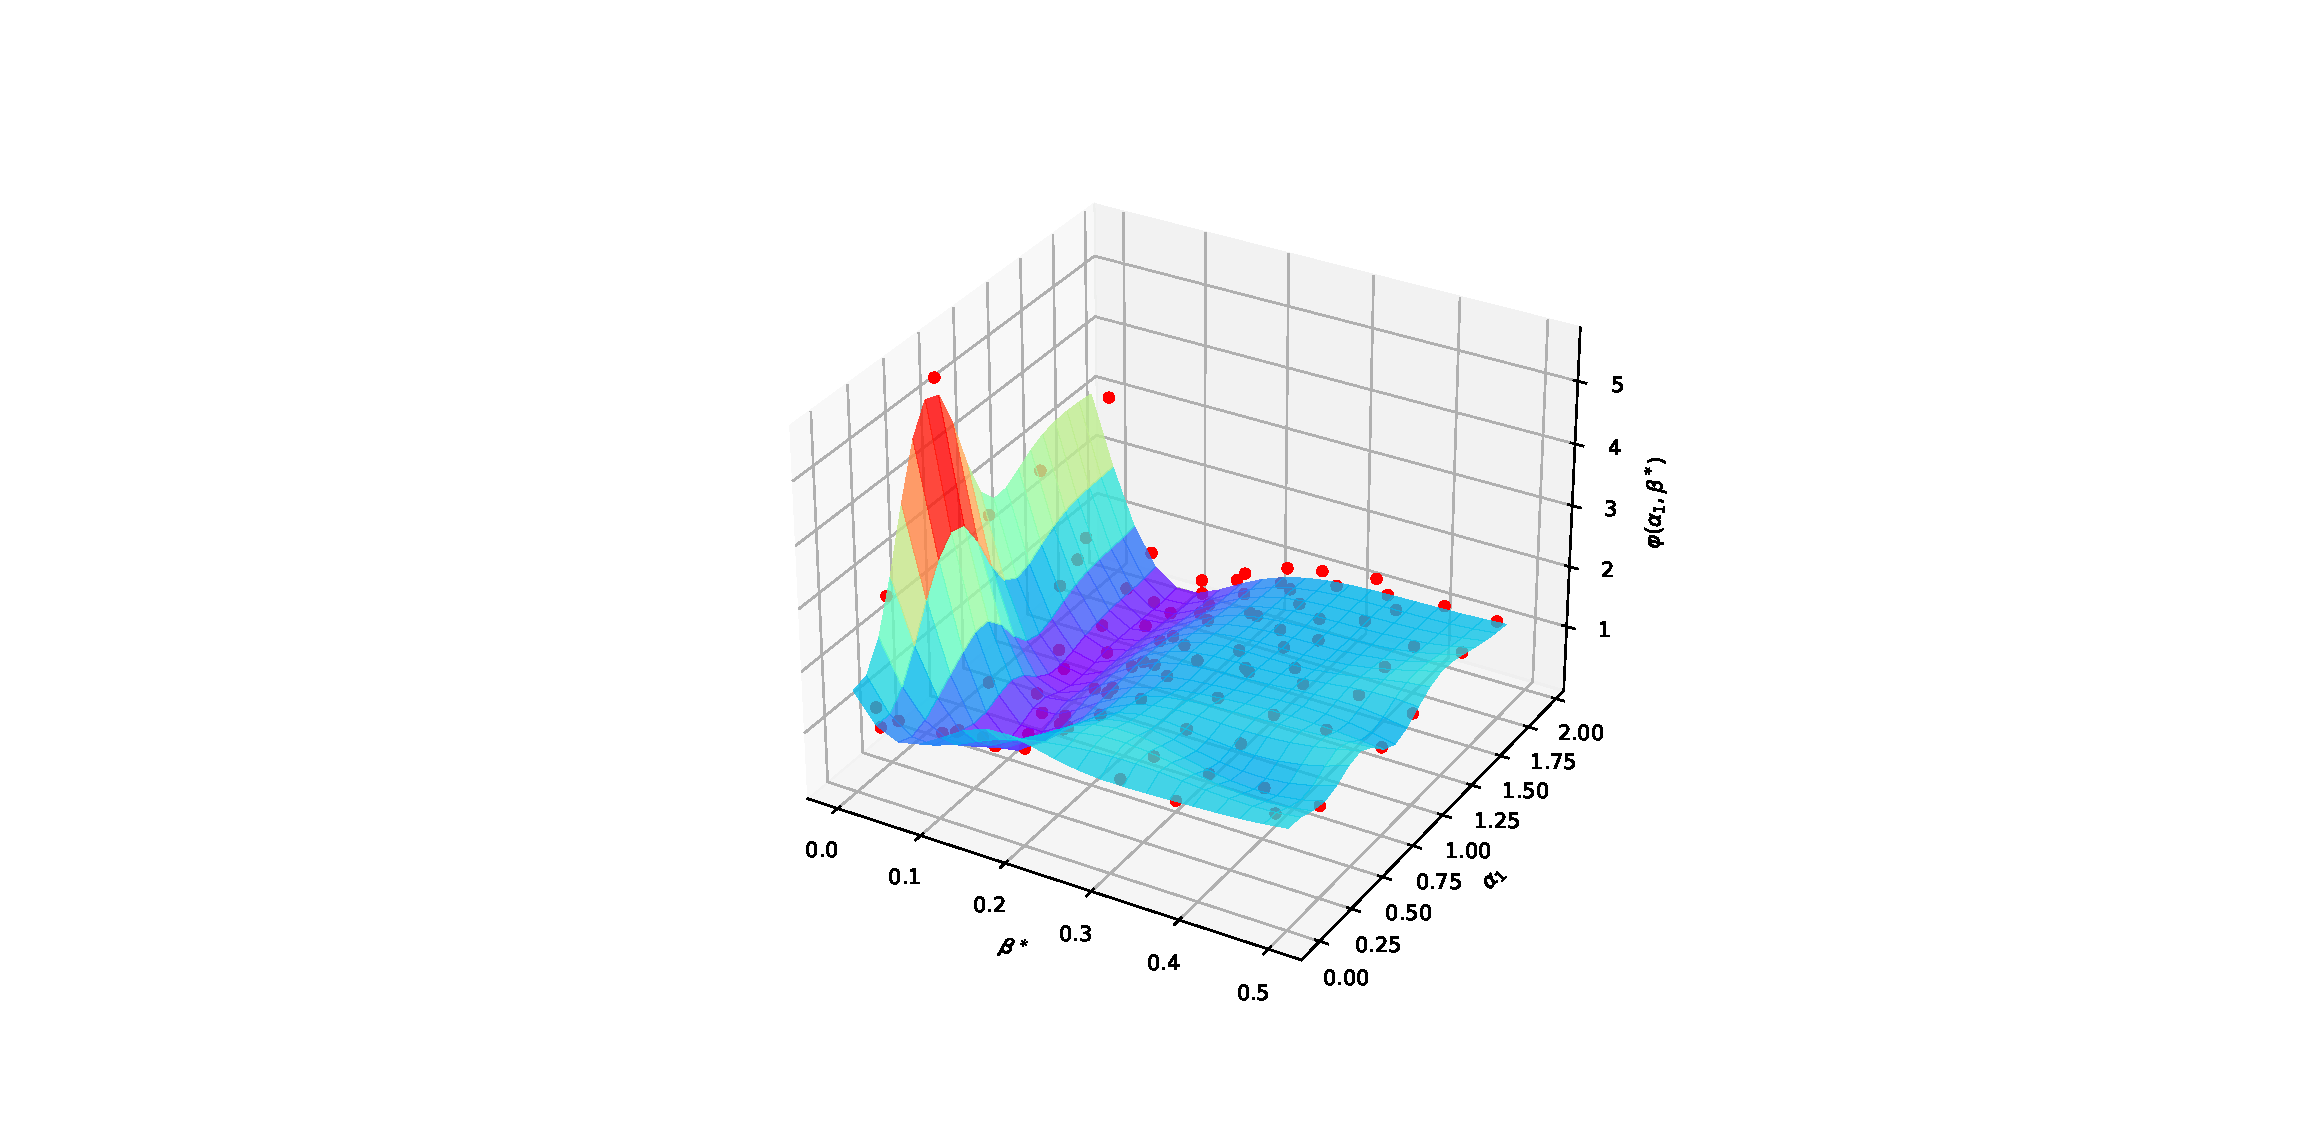
\includegraphics[width=0.6\linewidth]{NN_100_point_.pdf}
\caption{Задача значения функции (красные точки) и график аппроксимации, построенный с помощью нейронной сети (параметры $\beta^*$ и $a_1$ варьировались).\label{NN_100_point}}
 
\end{figure}   
 

Найденные лучшие значения параметров $\beta^*$ и $a_1$ были зафиксированы, после чего проводилась оптимизация по параметрам $\alpha_{k1}, \alpha_{\omega1}$ и $\alpha_{k2}, \alpha_{ \omega2}$.
Однако существенного улучшения целевой функции за счет оптимизации по этим параметрам добиться не удалось: было получено значение 0,365.


%На рисунках ~\ref{NN_100_point1} и ~\ref{NN_100_point2} приведены изображение функций, полученные с помощью аппроксимации задачи нейросетью, обученной на 100 точках испытания, варьировались соответсвенно пары параметров $\alpha_{k1} $,  $\alpha_{\omega1} $ и $\alpha_{k2} $, $\alpha_{\omega2} $.
%
%\begin{figure}[H]
%\begin{center}
%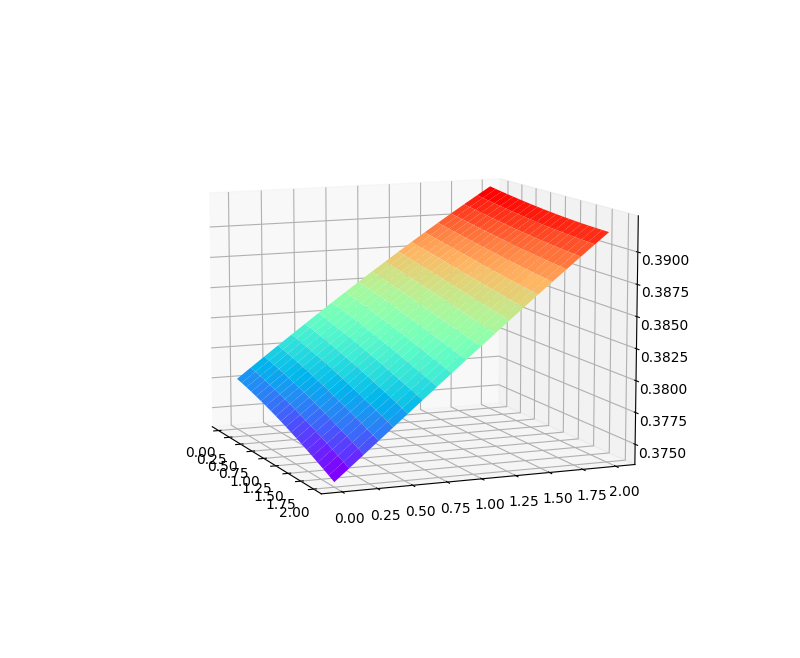
\includegraphics[width=1.0\linewidth]{ NN_100_point_1.png}
%\caption{Изображение функции, полученной с помощью аппроксимации задачи нейросетью, обученной на 100 точках испытания, варьировались параметры $\alpha_{k1} $ и $\alpha_{\omega1} $}
%\label{NN_100_point1}
%\end{center}
%\end{figure}
%
%\begin{figure}[H]
%\begin{center}
%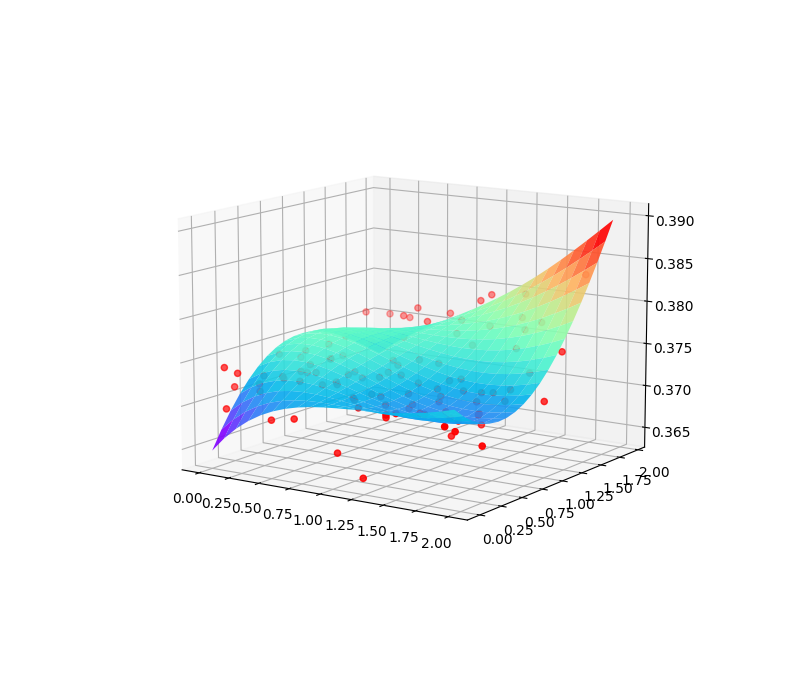
\includegraphics[width=1.0\linewidth]{ NN_100_point_tanh_alpha2_0.0001_.png}
%\caption{Изображение функции, полученной с помощью аппроксимации задачи нейросетью, обученной на 100 точках испытания, варьировались параметры $\alpha_{k2} $ и $\alpha_{\omega2} $}
%\label{NN_100_point2}
%\end{center}
%\end{figure}

%После калибровки значения коэффициентов стали следующими:
%The optimized values of the coefficients:
В итоге были получены следующие значения коэффициентов модели:

\begin{linenomath}
\begin{equation}
	\begin{aligned}
		\beta^* = 0.117;\ \ \ a_1 = 1.84;\ \ \ \alpha_{k 1} = 1.999;\\
		\alpha_{\omega 1} = 0.062; \ \ \ \alpha_{k 2} = 1.241;\ \ \ \alpha_{\omega 2} = 0.003.
	\end{aligned}
\end{equation}
\end{linenomath}

%Были получены следующие профили скорости на выходной плоскости для различных углов наклона лотка, как показано на рис.~\ref{NIIMexUProfilesKWSSTGlob}
На рис.~\ref{NIIMexUProfilesKWSSTGlob} показаны результирующие профили скорости $\bar{ {u_x}}$ в зависимости от глубины потока $h$ на выходной плоскости для различных углов наклона.

\begin{figure}[H]
\begin{adjustwidth}{-\extralength}{0cm}
\centering
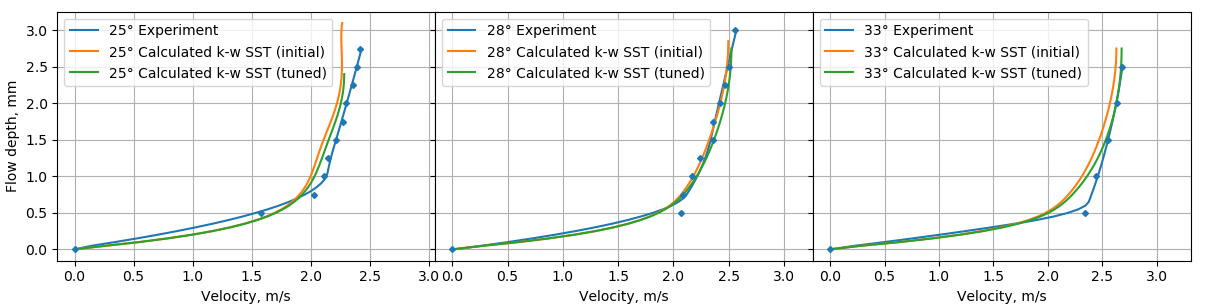
\includegraphics[width=18 cm]{UProfilesKWSSTGlob1.png}
\end{adjustwidth}
\caption{Графики сравнения экспериментального профиля скорости и расчетного профиля скорости с использованием стандартных значений коэффициентов модели турбулентности $k-\omega\ SST$ и расчетного профиля скорости с калиброванными значениями коэффициентов для различных углов наклона склона.\label{NIIMexUProfilesKWSSTGlob}}
\end{figure}  

%Калибровка привела к следующей минимизации функции потерь~\eqref{LossFunction}, показанной в таб.~\ref{tabLossFunctionMinimize}
В процессе калибровки была достигнута минимизация функции потерь~\eqref{LossFunction}, как показано в таблице~\ref{tabLossFunctionMinimize}.

%\begin{table}[H]
%	\caption{Минимизация функции потерь}
%	\label{tabLossFunctionMinimize}
%	\begin{center}
%		\begin{tabular}{ | c | m{0.3\textwidth} | m{0.3\textwidth} | } 
%			\hline
%			Угол наклона лотка& Начальное значение функции потерь & Минимизированное значение функции потерь\\
%			\hline
%			25$^\circ$ & 0.165 & 0.155\\
%			\hline
%			28$^\circ$ & 0.085 & 0.128\\
%			\hline
%			33$^\circ$ & 0.150 & 0.089\\
%			\hline
%		\end{tabular}
%	\end{center}
%\end{table}
\begin{table}[H] 
\caption{Значения функции потерь, полученные в процессе минимизации.\label{tabLossFunctionMinimize}}
\newcolumntype{C}{>{\centering\arraybackslash}X}
\begin{tabularx}{\textwidth}{CCC}
\toprule
    \textbf{Угол наклона склона} & \textbf{Начальное значение функции потерь} & \textbf{Значение функции минимальных потерь}\\
\midrule
    25$^\circ$ & 0.165 & 0.155\\
    28$^\circ$ & 0.085 & 0.128\\
    33$^\circ$ & 0.150 & 0.089\\
\bottomrule
\end{tabularx}
\end{table}
 

На рисунке \ref{NIIMexUProfilesKWSSTGlob} и в таблице \ref{tabLossFunctionMinimizeKE} можем видеть, что для двух углов наклона из трёх мы видим уменьшение расхождения расчётного профиля скорости с экспериментальным. Оптимизация по трём экспериментам одновременно (их функции потерь суммировались) использовалась с целью избежать переобучения модели, так как при использовании одного эксперимента, может быть достигнуто почти идеальное совпадение расчётного профиля скорости с экспериментальным, которое не воспроизводится на других экспериментах. Так же стоит отметить, что расхождение профиля скорости в области вблизи дна обусловлено погрешностью измерений в эксперименте, так как замер скорости с помощью трубки Пито, используемой в данном эксперименте, в непосредственной близости ото дна затруднён.


Минимальное значение целевой функции было получено при угле наклона 33 градуса. Одно вычисление целевой функции для заданных параметров занимало в среднем 15 минут с использованием 8 процессов MPI на узле суперкомпьютера Университета Лобачевского. Общее время расчета составило 24 часа.


%%%%%%%%%%%%%%%%%%%%%%%%%%%%%%%%%%%%%%%%%%
\section{Discussion}\label{sec6}

%В процессе работы над оптимизацией коэффициентов турбулентной модели мы столкнулись с рядом задач: создание интерфейса взаимодействия программного обеспечения Глобалайзер и пакета OpenFOAM; в процессе оптимизации мы столкнулись с проблемой переобучением модели; было проведено исследование наилучшей функции потерь и др.
When working on the optimization of the turbulent model coefficients, we faced a number of tasks: creating an interface for automatic interaction between the Globalizer software and the OpenFOAM package; in the process of optimization, we encountered the overfitting problem; and the study of the best loss function was carried out, etc.

%Создание интерфейса взаимодействия между Globalizer и OpenFOAM потребовало использования библиотеки pyFoam для подготовки прогонов расчетов. С помощью скрипта этой библиотеки pyFoamPrepareCase.py в расчетные варианты были записаны новые значения констант модели турбулентности, предложенной программой Globalizer. Далее проводился расчет в параллельном режиме и оценка полученного результата. Результат оценивался с помощью python-скрипта, который сравнивал полученный профиль скорости с экспериментальным.
Creating an interaction interface between Globalizer and OpenFOAM required the use of the pyFoam library to prepare calculation runs. Using the script of this library pyFoamPrepareCase.py, new values of the turbulent model coefficients proposed by the Globalizer software were written into the calculation cases. Next, the calculation was carried out in parallel mode and the result was evaluated using a python script that compared the obtained velocity profile with the experimental one.

A study of various loss functions has been carried out. The loss functions that estimate the absolute error of the velocity profile and the relative error were compared. The relative loss function actually penalizes the area near the bottom more, however, optimization using this loss function did not show significant improvements in the result. This behavior of the calculation is not due to the shortcomings of the numerical model, but rather due to the impossibility of taking velocity values correctly in the region very close to the bottom of the chute. It should be noted that measurements at the point closest to the bottom can have a significant error, due to the measurement method used (the Pitot tube). However, most of the profile was measured quite accurately, since for each measurement point in this stationary experiment, time averaging of 10 s was used. As a result of this study, it was decided to use the absolute loss function, since it showed the best optimization result.

We performed three experiments to avoid overfitting. It was noticed that when optimizing for one velocity profile, the algorithm perfectly calibrated the model, but for other experiments, the result was much worse. When optimizing for three experiments at once, this effect was avoided. The use of the obtained values of the coefficients for fluid flows that are close in dimensionless characteristics will allow a more accurate calculation to be made. However, when generalized to such canonical flows as air flow around different profiles, the use of the obtained values of the turbulent model coefficients is unlikely to show the best result.

\newpage

This study is part of a larger research effort related to the modeling of currents on the slopes of mountains. These flows are very difficult to study, since they are turbulent multi-phase flows of a non-Newtonian fluid on slopes of complex geometry. For such flows, the use of turbulent models using standard values of coefficients does not predict the flow in the best way. It is necessary to calibrate the turbulence model coefficients or create new turbulence models. We are considering both options. Moreover, a new turbulent model is being developed based on the neural network. However, the use of neural networks requires hybrid computing clusters, which is not always possible. As a result, it is important to be able to obtain a solution of sufficient accuracy using the classical turbulent model. This problem requires the calibration of the coefficients, which was done in this work for the Newtonian medium. Optimization algorithms were developed and tested, which can later be used to calibrate the coefficients of any turbulent models. The next stage of the study is to set up an experiment with a non-Newtonian fluid and calibrate the coefficients of the turbulent model according to the developed algorithm.

%Отметим также, что при поиске оптимальных параметров модели проводилась оптимизация сначала по параметрам $\beta^*$ and $a_1$, затем – по параметрам $\alpha_{k1}, \alpha_{\omega1}$, and $\alpha_{k2}, \alpha_{\omega2}$. Данный способ позволил найти хорошее решение за приемлемое время. Поиск глобального минимума сразу по всем варьируемым параметрам потребовал бы на порядки большего числа испытаний и, соответственно, времени. Указанный эффект ключевым образом отличает задачи глобальной оптимизации от задач на локальный экстремум, в которых затраты растут не столь быстро.
We also note that when searching for the optimal model parameters, optimization was carried out first with respect to the parameters $\beta^*$ and $a_1$, then optimization in $\alpha_{k1}, \alpha_{\omega1}$, and $\alpha_{k2}, \alpha_{\omega2}$ was performed. This approach makes it possible to find a good solution in a reasonable amount of time.
The search for a global optimum for all parameters at once would require orders of magnitude more trials and time.
This effect is a key difference between global optimization and local optimization problems, in which the costs do not grow as fast.

%С точки зрения решения вычислительно трудоемкой задачи оптимизации с целевой функцией вида черный ящик представляет интерес сравнение использованного метода решения задачи, в котором целевая функция аппроксимировалась нейросетью, с распространенными методами, использующими аппроксимации на основе кригинга. Методы данного класса хорошо работают в задачах с небольшим числом локальных экстремумов, однако в существенно многоэкстремальных задачах вычислительные затраты значительно возрастают.
In terms of solving a time-consuming optimization problem with a black-box objective function, it is interesting to compare the method used for solving the problem, which uses objective function approximation by a neural network, with the methods that use kriging-based approximations.
Methods of this class work well in problems with a small number of local extrema.
However, in essentially multi-extremal problems the computational costs (number of objective function evaluations required for solving the problem) increase significantly.


%%%%%%%%%%%%%%%%%%%%%%%%%%%%%%%%%%%%%%%%%%
\section{Conclusions}\label{sec7}

In this work, a two-phase flow in a chute was simulated using the interFoam solver, the URANS mathematical model, and the $k-\omega\ SST$ turbulence model. In the optimization process, six coefficients were investigated in pairs, which make the greatest contribution to the value of turbulent viscosity.

The results of calculating the velocity profiles were compared with experimental data obtained at the Research Institute of Mechanics, Moscow State University, at different sections depending on the angle of inclination of the chute. The search for the optimal coefficients of the turbulence model was performed by minimizing the objective function of the divergence of the velocity profile in the chute. % - RMSE.

The search for the global minimum of the objective function was performed using the global search algorithm implemented in the Globalizer software~\cite{globalizerSystem}. In addition, a fully connected neural network with one hidden layer was used to approximate the values of the objective function by the values of the coefficients in the turbulence model. The MLPRegressor class from the scikit-learn library was used to build the objective function approximation.

Based on the results of the study, the following conclusions were drawn.

It is good practice to calibrate the turbulence model coefficients if necessary to improve the accuracy of the calculations. As shown in the present study, it is possible to improve the accuracy by up to 10\%.

To perform optimization, at least two, or preferably three datasets should be used. Otherwise, an overfitted model may result.
Using a neural network to predict the CFD calculation significantly reduced the optimization time while maintaining the quality of the resulting solution.

 

The developed calibration algorithm is reliable and can be applied to other models. The algorithm has such advantages as a parallel mode, it can be used to search not only for local, but also for global minima, and can optimize several parameters at once. According to the results of the study, the Globalizer software has performed quite well and will be used in further work.

The OpenFOAM software also shows good results due to code modularity and good documentation. These advantages have made it easier to write a software module for the interaction between the optimizer and OpenFOAM. OpenFOAM also has a high degree of parallelization and can be used to solve a fairly wide range of tasks.

In the present work, an interdisciplinary approach was utilized, which helped us to find the optimal values of six turbulence model parameters using the OpenFOAM open platform and the Globalizer.  
In the future, it is planned to continue improving the turbulent models, including the development of a turbulent model based on a neural network. The Globalizer software will be used to optimize the model parameters.

\nomenclature{NNR		}{ Neural Network Regression	}
\nomenclature{RMSE		}{ Root-Mean-Square Error	}
\nomenclature{CFD }{ Computational Fluid Dynamic }
\nomenclature{RANS }{ Reynolds-Averaged Navier-Stokes equations }
\nomenclature{PISO }{ Pressure Implicit with Splitting of Operator }
\nomenclature{SIMPLE }{ Semi-Implicit Method for Pressure-Linked Equations }
\nomenclature{PIMPLE }{ combination of PISO and SIMPLE }  

%%%%%%%%%%%%%%%%%%%%%%%%%%%%%%%%%%%%%%%%%%
\vspace{6pt} 

%%%%%%%%%%%%%%%%%%%%%%%%%%%%%%%%%%%%%%%%%%
%% optional
%\supplementary{The following supporting information can be downloaded at:  \linksupplementary{s1}, Figure S1: title; Table S1: title; Video S1: title.}

% Only for the journal Methods and Protocols:
% If you wish to submit a video article, please do so with any other supplementary material.
% \supplementary{The following supporting information can be downloaded at: \linksupplementary{s1}, Figure S1: title; Table S1: title; Video S1: title. A supporting video article is available at doi: link.}

%%%%%%%%%%%%%%%%%%%%%%%%%%%%%%%%%%%%%%%%%%
\authorcontributions{Conceptualization, K.B. and D.R. (Daniil Ryazanov); methodology, D.R. (Daria Romanova) and K.B.; software, I.L., D.R. (Daniil Ryazanov), M.U., and  D.R. (Daria Romanova); validation,  D.R. (Daria Romanova) and I.L.; formal analysis, S.S., M.U.; investigation, S.S.; resources, I.L.; data curation, D.R. (Daria Romanova) and M.U.; writing---original draft preparation, K.B., S.S. and D.R. (Daria Romanova); writing---review and editing, D.R. (Daniil Ryazanov); visualization, I.L.; supervision, S.S.; project administration, K.B.; funding acquisition, S.S. All authors have read and agreed to the published version of the manuscript.}

\funding{This research was supported by the Ministry of Science and Higher Education of the Russian Federation, agreement No 075-15-2020-808.}

\institutionalreview{Not applicable.}

\informedconsent{Not applicable.}

\dataavailability{Not applicable.} 

\acknowledgments{The authors consider it their duty to acknowledge the contribution of  Victor Gergel (14.01.1955--29.06.2021), who initiated this interdisciplinary study.}

\conflictsofinterest{The authors declare no conflicts of interest.} 

%%%%%%%%%%%%%%%%%%%%%%%%%%%%%%%%%%%%%%%%%%
%% Optional
%\sampleavailability{Samples of the compounds ... are available from the authors.}

%% Only for journal Encyclopedia
%\entrylink{The Link to this entry published on the encyclopedia platform.}

%\abbreviations{Abbreviations}{
%The following abbreviations are used in this manuscript:\\

%\noindent 
%\begin{tabular}{@{}ll}
%MDPI & Multidisciplinary Digital Publishing Institute\\
%DOAJ & Directory of open access journals\\
%TLA & Three letter acronym\\
%LD & Linear dichroism
%\end{tabular}
%}

%%%%%%%%%%%%%%%%%%%%%%%%%%%%%%%%%%%%%%%%%%
%% Optional
\appendixtitles{no} % Leave argument "no" if all appendix headings stay EMPTY (then no dot is printed after "Appendix A"). If the appendix sections contain a heading then change the argument to "yes".

%%\appendixstart
%%\appendix
%%\section[\appendixname~\thesection]{}\label{app}%Nomenclature%List of symbols and abbreviations


%\subsection[\appendixname~\thesubsection]{}
%The appendix is an optional section that can contain details and data supplemental to the main text---for example, explanations of experimental details that would disrupt the flow of the main text but nonetheless remain crucial to understanding and reproducing the research shown; figures of replicates for experiments of which representative data are shown in the main text can be added here if brief, or as Supplementary Data. Mathematical proofs of results not central to the paper can be added as an appendix.

%$\alpha_{k1,2}$, $\alpha_{\omega1,2}$, $\beta_{1,2}$, $\gamma_{1,2}$, $\beta^*$, $a_1$, $b_1$, $c_1$ & turbulence model constant \\

%%\vspace{-6pt}

%%\begin{table}[H] 
%%\caption{\hl{Nomenclature}.\label{A:tab1}} 
%MDPI: Please consider using  Nomenclature format instead, Not Appendix A, Table A1
%Authors: The nomenclature has been revised. But we think it looks better in tables. Therefore, we have left the tables here as a comment with double commenting symbol (&&).
%%\newcolumntype{C}{>{\centering\arraybackslash}X}
%%\begin{tabularx}{\textwidth}{ll}
%%\toprule
%%$u_0$		& depth-averaged velocity on the inlet plane of the experiment chute	\\
%%$h_0$		& flow depth on the inlet plane of the experiment chute	\\
%%$\theta$	& inclination angle of the experiment chute \\
%%$\alpha$	& water volume fraction	\\
%%$\bar{ {\tau}}$	& Reynolds-averaged stress tensor	\\
%%$\bar{ {s}}$		& Reynolds-averaged strain rate tensor	\\
%%$\mu_{eff}$		& effective viscosity	\\
%%$\mu$		& molecular viscosity	\\
%%$\mu_{t}$		& turbulent viscosity	\\
%%$\bar{ {f}}$		& Reynolds-averaged density of body forces	\\
%%$\bar{ {u}}$		& Reynolds-averaged velocity of the mixture	\\
%%$\rho$		& density of the mixture	\\
%%$\bar{p}$		& pressure of the mixture	\\
%%$\omega$		& specific dissipation rate of the turbulent kinetic energy	\\
%%$k$		& 	turbulent kinetic energy \\
%%$F_1$		& first blending function	\\
%%$\dot{ {s}}$		& Reynolds-averaged strain rate	\\
%%$F_2$		& second blending function	\\
%%$\widetilde{P}_k$ & the limiter on the growth of turbulence used in stagnation modes \\
%%$\alpha_k$ & turbulence model closure coefficient \\
%%$\alpha_{k1}$ & turbulence model closure coefficient \\
%%$\alpha_{k2}$ & turbulence model closure coefficient \\
%%$\alpha_\omega$ & turbulence model closure coefficient \\
%%$\alpha_{\omega1}$ & turbulence model closure coefficient \\
%%$\alpha_{\omega2}$ & turbulence model closure coefficient \\
%%$\beta$ & turbulence model closure coefficient \\
%%$\beta_1$ & turbulence model closure coefficient \\
%%$\beta_2$ & turbulence model closure coefficient \\
%%$\gamma$ & turbulence model closure coefficient \\
%%$\gamma_1$ & turbulence model closure coefficient \\
%%$\gamma_2$ & turbulence model closure coefficient \\
%%$\beta^*$ & turbulence model closure coefficient \\
%%$a_1$ & turbulence model closure coefficient \\
%%$b_1$ & turbulence model closure coefficient \\
%%$c_1$ & turbulence model closure coefficient \\
%%$y = (y_1, ..., y_N)$ & vector of parameter\\
%%$\varphi(y)$		& objective function	\\
%%$D$	& hyperinterval	\\
%%$N$		& number of measuring points of velocity over the flow depth at the outlet plane	\\
%%$u^i_{EXP}$		& horizontal component of velocity at the control point obtained by experiment	\\
%%$u^i_{k-\omega}\ SST$		& horizontal component of velocity at the control point calculated by CFD	\\
%%$ {L_{RMSE}}$		& loss function	\\
%%$L$		& Lipschitz constant	\\
%%$H$		& H{\"o}lder constant	\\
%%$y(x)$		& Peano curve	\\
%%$f(x) = \varphi(y(x))$		& univariate function	\\
%%$X_k=\{x^0,\dots,x^k\} $ & set of the trial points \\
%%$z^k = f(x^k)$ & value of the objective function \\
%%$M$		& adaptive estimation of the Lipschitz constant \\
%%$R(i)$		& characteristic of the $i$-th search interval\\
%%$r>0$		& method parameter	\\
%%$\epsilon > 0$		& search accuracy	\\
%%$\Omega $ & set of the trial results \\
%%$\overline{\varphi}(y)$ & approximation of the objective function \\
%%\bottomrule
%%\end{tabularx}
%%\end{table}

%%\begin{table}[H] 
%%\caption{\hl{List of abbreviations.}\label{A:tab2}} %MDPI: Please consider using  Abbreviations format instead, Not Appendix A, Table A2. 
%%\newcolumntype{C}{>{\centering\arraybackslash}X}
%%\begin{tabularx}{\textwidth}{ll}
%%\toprule
%%NNR		& Neural Network Regression	\\
%%RMSE		& Root-Mean-Square Error	\\
%%CFD & Computational Fluid Dynamic \\
%%RANS & Reynolds-Averaged Navier-Stokes equations \\
%%PISO & Pressure Implicit with Splitting of Operator \\
%%SIMPLE & Semi-Implicit Method for Pressure-Linked Equations \\
%%PIMPLE & combination of PISO and SIMPLE \\  
%%\bottomrule
%%\end{tabularx}
%%\end{table}

%\section[\appendixname~\thesection]{}
%All appendix sections must be cited in the main text. In the appendices, Figures, Tables, etc. should be labeled, starting with ``A''---e.g., Figure A1, Figure A2, etc.

\printnomenclature

%%%%%%%%%%%%%%%%%%%%%%%%%%%%%%%%%%%%%%%%%%
\begin{adjustwidth}{-\extralength}{0cm}
%\printendnotes[custom] % Un-comment to print a list of endnotes

\reftitle{References}

% Please provide either the correct journal abbreviation (e.g., according to the “List of Title Word Abbreviations” http://www.issn.org/services/online-services/access-to-the-ltwa/) or the full name of the journal.
% Citations and References in Supplementary files are permitted provided that they also appear in the reference list here. 

%=====================================
% References, variant A: external bibliography
%=====================================
%\bibliography{your_external_BibTeX_file}
\begin{thebibliography}{999}

\bibitem[Pendin and Fomenko(2015)]{Pendin2015}
Pendin, V.; Fomenko, I.
\newblock {\em Landslide Hazard Assessment and Prediction Methodology};  2015; 
  p. 320. 
  %MDPI: Please add the name of the publisher and the location (city, country) of it. Or please add website and accessed date(before receive date 6 July 2022)
  %Authors: Information is not available

\bibitem[Froude and Petley(2018)]{Froude2018}
Froude, M.J.; Petley, D.N.
\newblock Global fatal landslide occurrence from 2004 to 2016.
\newblock {\em Nat. Hazards Earth Syst. Sci.} {\bf 2018}, {\em
  18},~2161--2181.
\newblock {{https://doi.org/10.5194/nhess-18-2161-2018}}.

\bibitem[Hungr(2005)]{hungr2005landslide}
Hungr, O.
\newblock {\em Landslide Risk Management: Proceedings of the International
  Conference on Landslide Risk Management, Vancouver, BC,  Canada, 31 May--3 June
  2005}; Balkema: Leiden, NY, USA,  2005.

\bibitem[Kharchenko and Shvarev(2020)]{Harch2020}
Kharchenko, S.; Shvarev, S.
\newblock Forecasting of Landslide Hazards in the Vicinity of Krasnaya Polyana
  Basing on Liniar Discriminatory Analysis.
\newblock {\em Vestnik Moskow State Univ. Ser. 5 Geography.} {\bf 2020},  22--33.
\newblock
  Available online:  \url{https://vestnik5.geogr.msu.ru/jour/article/view/668?locale=en_US}  accessed on 1 may 2022).
  %MDPI: Please add volume and doi link.  Or please add website and accessed date(before receive date 6 July 2022)
  %Authors: Fixed

\bibitem[Bernander \em{et~al.}(2016)Bernander, Kullingsj\"{o}, Gylland,
  Bengtsson, Knutsson, Pusch, Olofsson, and Elfgren]{Bernander2016}
Bernander, S.; Kullingsj\"{o}, A.; Gylland, A.S.; Bengtsson, P.E.; Knutsson,
  S.; Pusch, R.; Olofsson, J.; Elfgren, L.
\newblock Downhill progressive landslides in long natural slopes: Triggering
  agents and landslide phases modeled with a finite difference method.
\newblock {\em Can. Geotech. J.} {\bf 2016}, {\em 53},~1565--1582.
\newblock {{https://doi.org/10.1139/cgj-2015-0651}}.

\bibitem[Gao \em{et~al.}(2007)Gao, Jian-li, and Chang-yu]{liu2007application}
Gao, L.; Jian-li, D.; Chang-yu, L.
\newblock The application of finite volume method to modeling landslide motion.
\newblock {\em Adv. Earth Sci.} {\bf 2007}, {\em 22},~1129--1133.

\bibitem[Liu \em{et~al.}(2020)Liu, Su, Zhang, Iqbal, Hu, and Dong]{Liu2020}
Liu, Z.; Su, L.; Zhang, C.; Iqbal, J.; Hu, B.; Dong, Z.
\newblock Investigation of the dynamic process of the Xinmo landslide using the
  discrete element method.
\newblock {\em Comput. Geotech.} {\bf 2020}, {\em 123},~103561.
\newblock {{https://doi.org/10.1016/j.compgeo.2020.103561}}.

\bibitem[Piegari \em{et~al.}(2006)Piegari, Cataudella, Di~Maio, Milano, and
  Nicodemi]{piegari2006cellular}
Piegari, E.; Cataudella, V.; Di~Maio, R.; Milano, L.; Nicodemi, M.
\newblock A cellular automaton for the factor of safety field in landslides
  modeling.
\newblock {\em Geophys. Res. Lett.} {\bf 2006}, {\em 33}, L01403.

\bibitem[Hirt and Nichols(1981)]{Hirt1981}
Hirt, C.; Nichols, B.
\newblock Volume of fluid ({VOF}) method for the dynamics of free boundaries.
\newblock {\em J. Comput. Phys.} {\bf 1981}, {\em
  39},~201--225. 
  %MDPI: Ref. 9 and 68 are same.  please, either replace the duplicate with a new reference, or we will help remove the duplicate and rearrange the reference order.
  %Authors: Fixed
\newblock {{https://doi.org/10.1016/0021-9991(81)90145-5}}.

\bibitem[Naaim \em{et~al.}(2002)Naaim, Furdada, and Mart{\'{\i}}nez]{Naaim2002}
Naaim, M.; Furdada, G.; Mart{\'{\i}}nez, H.
\newblock Calibration and application of the {MN}2D dynamics model to the
  avalanches of Las Le{\~{n}}as (Argentina).
\newblock {\em Nat. Hazards Earth Syst. Sci.} {\bf 2002}, {\em
  2},~221--226.
\newblock {{https://doi.org/10.5194/nhess-2-221-2002}}.

\bibitem[Pitman \em{et~al.}(2003)Pitman, Nichita, Patra, Bauer, Sheridan, and
  Bursik]{Pitman2003}
Pitman, E.B.; Nichita, C.C.; Patra, A.; Bauer, A.; Sheridan, M.; Bursik, M.
\newblock Computing granular avalanches and landslides.
\newblock {\em Phys. Fluids} {\bf 2003}, {\em 15},~3638--3646.
\newblock {{https://doi.org/10.1063/1.1614253}}.

\bibitem[Oda \em{et~al.}(2011)Oda, Moriguchi, Kamiishi, Yashima, Sawada, and
  Sato]{Oda2011}
Oda, K.; Moriguchi, S.; Kamiishi, I.; Yashima, A.; Sawada, K.; Sato, A.
\newblock Simulation of a snow avalanche model test using computational fluid
  dynamics.
\newblock {\em Ann. Glaciol.} {\bf 2011}, {\em 52},~57--64.
\newblock {{https://doi.org/10.3189/172756411797252284}}.

\bibitem[Yamaguchi \em{et~al.}(2017)Yamaguchi, Takase, Moriguchi, Terada, Oda,
  and Kamiishi]{Yamaguchi2017}
Yamaguchi, Y.; Takase, S.; Moriguchi, S.; Terada, K.; Oda, K.; Kamiishi, I.
\newblock Three-dimensional nonstructural finite element analysis of snow
  avalanche using non-Newtonian fluid model.
\newblock {\em Trans. Jpn. Soc. Comput. Eng. Sci.} {\bf 2017}, {\em 2017}, 20170011.
\newblock {{https://doi.org/10.11421/jsces.2017.20170011}}.

\bibitem[Agustsdottir(2019)]{IceThesKatr}
Agustsdottir, K.H.
\newblock The Design of Slushflow Barriers: Laboratory Experiments. Doctoral Dissertation, University of Iceland,  Reykjavik, Iceland, 
\newblock  2019.

\bibitem[Jones(2019)]{IceThesJon}
Jones, R.
\newblock The Design of Slushflow Barriers: CFD Simulations. Doctoral Dissertation,
\newblock  2019.
%MDPI: Please add Degree-Granting University and Location of University(city and countrty).  Or please add website and accessed date(before receive date 6 July 2022)
%Authors: Fixed
\newblock
  Available online:  \url{http://hdl.handle.net/1946/34502}  accessed on 1 may 2022).

\bibitem[Jaedicke \em{et~al.}(2006)Jaedicke, Kern, Gauer, Baillifard, and
  Platzer]{Jaedicke2006}
Jaedicke, C.; Kern, M.; Gauer, P.; Baillifard, M.A.; Platzer, K.
\newblock Chute Experiments on Slushflow Dynamics. In  Proceedings of the   2006 International Snow Science Workshop,  Telluride, CO, USA, 1--6 October 2006.
\newblock  

\bibitem[Cheung \em{et~al.}(2011)Cheung, Oliver, Prudencio, Prudhomme, and
  Moser]{Cheung2011}
Cheung, S.H.; Oliver, T.A.; Prudencio, E.E.; Prudhomme, S.; Moser, R.D.
\newblock Bayesian uncertainty analysis with applications to turbulence
  modeling.
\newblock {\em Reliab. Eng.  Syst. Saf.} {\bf 2011}, {\em
  96},~1137--1149.
\newblock {{https://doi.org/10.1016/j.ress.2010.09.013}}.

\bibitem[Guillas \em{et~al.}(2014)Guillas, Glover, and
  Malki-Epshtein]{Guillas2014}
Guillas, S.; Glover, N.; Malki-Epshtein, L.
\newblock Bayesian calibration of the constants of the turbulence model for a
  {CFD} model of street canyon flow.
\newblock {\em Comput. Methods Appl. Mech. Eng.} {\bf
  2014}, {\em 279},~536--553.
\newblock {{https://doi.org/10.1016/j.cma.2014.06.008}}.

\bibitem[Edeling \em{et~al.}(2014{\natexlab{a}})Edeling, Cinnella, and
  Dwight]{Edeling2014a}
Edeling, W.; Cinnella, P.; Dwight, R.
\newblock Predictive {RANS} simulations via Bayesian Model-Scenario Averaging.
\newblock {\em J. Comput. Phys.} {\bf 2014}, {\em 275},~65--91.
\newblock {{https://doi.org/10.1016/j.jcp.2014.06.052}}.

\bibitem[Edeling \em{et~al.}(2014{\natexlab{b}})Edeling, Cinnella, Dwight, and
  Bijl]{Edeling2014b}
Edeling, W.; Cinnella, P.; Dwight, R.; Bijl, H.
\newblock Bayesian estimates of parameter variability in the
  k{\textendash}$\upepsilon$ turbulence model.
\newblock {\em J. Comput. Phys.} {\bf 2014}, {\em 258},~73--94.
\newblock {{https://doi.org/10.1016/j.jcp.2013.10.027}}.

\bibitem[de~Zordo-Banliat \em{et~al.}(2020)de~Zordo-Banliat, Merle, Dergham,
  and Cinnella]{deZordoBanliat2020}
de~Zordo-Banliat, M.; Merle, X.; Dergham, G.; Cinnella, P.
\newblock Bayesian model-scenario averaged predictions of compressor cascade
  flows under uncertain turbulence models.
\newblock {\em Comput.  Fluids} {\bf 2020}, {\em 201},~104473.
\newblock {{https://doi.org/10.1016/j.compfluid.2020.104473}}.

\bibitem[Matsui \em{et~al.}(2021)Matsui, Perez, Kelly, Tani, and
  Jemcov]{Matsui2021}
Matsui, K.; Perez, E.; Kelly, R.; Tani, N.; Jemcov, A.
\newblock Calibration of Spalart-Allmaras model for simulation of corner flow
  separation in linear compressor cascade.
\newblock {\em J. Glob. Power Propuls. Soc.} {\bf 2021},
  pp. 1--16.
\newblock {{https://doi.org/10.33737/jgpps/135174}}.

\bibitem[Xiao and Cinnella(2019)]{Xiao2019}
Xiao, H.; Cinnella, P.
\newblock Quantification of model uncertainty in {RANS} simulations: A review.
\newblock {\em Prog. Aerosp. Sci.} {\bf 2019}, {\em 108},~1--31.
\newblock {{https://doi.org/10.1016/j.paerosci.2018.10.001}}.

\newpage

\bibitem[Karpatne \em{et~al.}(2017)Karpatne, Ebert{-}Uphoff, Ravela, Babaie,
  and Kumar]{GeoML}
Karpatne, A.; Ebert{-}Uphoff, I.; Ravela, S.; Babaie, H.A.; Kumar, V.
\newblock Machine Learning for the Geosciences: Challenges and Opportunities. \emph{IEEE Trans. Knowl. Data Eng.}  \textbf{2018}, \emph{31}, 1544--1554. %MDPI: We revised journal information, please confirm
%\newblock {\em CoRR} {\bf 2017}, {\em abs/1711.04708},
%  \href{http://xxx.lanl.gov/abs/1711.04708}{{\normalfont [1711.04708]}}.
%Authors: Ok

\bibitem[Ma \em{et~al.}(2020)Ma, Mei, and Piccialli]{Ma2020}
Ma, Z.; Mei, G.; Piccialli, F.
\newblock Machine learning for landslides prevention: A survey.
\newblock {\em Neural Comput. Appl.} {\bf 2020}, {\em
  33},~10881--10907.
\newblock {{https://doi.org/10.1007/s00521-020-05529-8}}.

\bibitem[Yu \em{et~al.}(2022)Yu, Wu, Wang, and Gu]{YuWuWang2022}
Yu, D.; Wu, J.; Wang, W.; Gu, B.
\newblock Optimal performance of hybrid energy system in the presence of
  electrical and heat storage systems under uncertainties using stochastic
  p-robust optimization technique.
\newblock {\em Sustain. Cities Soc.} {\bf 2022}, {\em 83},~103935.
\newblock {{https://doi.org/10.1016/j.scs.2022.103935}}.

\bibitem[Bagautdinov \em{et~al.}(2021)Bagautdinov, Wu, Simon, Prada, Shiratori,
  Wei, Xu, Sheikh, and Saragih]{BagautdinovWuSimon2021}
Bagautdinov, T.; Wu, C.; Simon, T.; Prada, F.; Shiratori, T.; Wei, S.E.; Xu,
  W.; Sheikh, Y.; Saragih, J.
\newblock Driving-Signal Aware Full-Body Avatars.
\newblock {\em ACM Trans. Graph.} {\bf 2021}, {\em 40}, 1--17.
\newblock {{https://doi.org/10.1145/3450626.3459850}}.

\bibitem[Zhang \em{et~al.}(2022)Zhang, Zhang, and Cai]{ZhangZhangCai2022}
Zhang, L.; Zhang, H.; Cai, G.
\newblock The Multiclass Fault Diagnosis of Wind Turbine Bearing Based on
  Multisource Signal Fusion and Deep Learning Generative Model.
\newblock {\em IEEE Trans. Instrum. Meas.} {\bf
  2022}, {\em 71},~1--12.
\newblock {{https://doi.org/10.1109/TIM.2022.3178483}}.

\bibitem[Zhang \em{et~al.}(2021)Zhang, Liu, Fang, Yuan, Zhang, and
  Lu]{ZhangLiuFang2021}
Zhang, Y.; Liu, F.; Fang, Z.; Yuan, B.; Zhang, G.; Lu, J.
\newblock Learning From a Complementary-Label Source Domain: Theory and
  Algorithms.
\newblock {\em IEEE Trans. Neural Netw. Learn. Syst.} {\bf
  2021}. 
  %MDPI: Please add volume and page if available
  %Authors: Information is not available
\newblock {{https://doi.org/10.1109/TNNLS.2021.3086093}}.

\bibitem[Zhong \em{et~al.}(2021)Zhong, Fang, Liu, Yuan, Zhang, and
  Lu]{ZhongFangLiu2021}
Zhong, L.; Fang, Z.; Liu, F.; Yuan, B.; Zhang, G.; Lu, J.
\newblock Bridging the Theoretical Bound and Deep Algorithms for Open Set
  Domain Adaptation.
\newblock {\em IEEE Trans. Neural Netw. Learn. Syst.} {\bf
  2021},  1--15. 
  %MDPI: Please add volume  if available
  %Authors: Information is not available
\newblock {{https://doi.org/10.1109/TNNLS.2021.3119965}}.

\bibitem[Maggiori \em{et~al.}(2017)Maggiori, Tarabalka, Charpiat, and
  Alliez]{Maggiori2017}
Maggiori, E.; Tarabalka, Y.; Charpiat, G.; Alliez, P.
\newblock Convolutional Neural Networks for Large-Scale Remote-Sensing Image
  Classification.
\newblock {\em {IEEE} Trans. Geosci. Remote Sens.} {\bf
  2017}, {\em 55},~645--657.
\newblock {{https://doi.org/10.1109/tgrs.2016.2612821}}.

\bibitem[Qin \em{et~al.}(2021)Qin, Guo, Sun, Qiao, Zhang, Yao, Cheng, and
  Zhang]{Qin2021}
Qin, S.; Guo, X.; Sun, J.; Qiao, S.; Zhang, L.; Yao, J.; Cheng, Q.; Zhang, Y.
\newblock Landslide Detection from Open Satellite Imagery Using Distant Domain
  Transfer Learning.
\newblock {\em Remote Sens.} {\bf 2021}, {\em 13},~3383.
\newblock {{https://doi.org/10.3390/rs13173383}}.

\bibitem[Prakash \em{et~al.}(2021)Prakash, Manconi, and Loew]{Prakash2021}
Prakash, N.; Manconi, A.; Loew, S.
\newblock A new strategy to map landslides with a generalized convolutional
  neural network.
\newblock {\em Sci. Rep.} {\bf 2021}, {\em 11}, 9722.
\newblock {{https://doi.org/10.1038/s41598-021-89015-8}}.

\bibitem[Menter(1993)]{Menter1993}
Menter, F. Zonal Two Equation k-w Turbulence Models For Aerodynamic Flows.
\newblock  In  Proceedings of the    23rd Fluid Dynamics, Plasmadynamics, and Lasers Conference,  Orlando, FL, USA,  6--9 July 1993.
\newblock {{https://doi.org/10.2514/6.1993-2906}}.

\bibitem[Menter(1994)]{Menter1994}
Menter, F.R.
\newblock Two-equation eddy-viscosity turbulence models for engineering
  applications.
\newblock {\em AIAA J.} {\bf 1994}, {\em 32},~1598--1605.
\newblock {{https://doi.org/10.2514/3.12149}}.

\bibitem[Menter \em{et~al.}(2003)Menter, Kuntz, and
  Langtry]{MenterKuntzLangtry2003}
Menter, F.; Kuntz, M.; Langtry, R.
\newblock Ten years of industrial experience with the SST turbulence model.
\newblock {\em Heat Mass Transf.} {\bf 2003}, {\em 4}, 625--632.

\bibitem[Matyushenko and Garbaruk(2016)]{MatyushenkoGarbaruk2016}
Matyushenko, A.A.; Garbaruk, A.V.
\newblock Adjustment of the k-$\omega$~SST turbulence model for prediction of
  airfoil characteristics near stall.
\newblock {\em J. Phys. Conf. Ser.} {\bf 2016}, {\em
  769},~012082.
\newblock {{https://doi.org/10.1088/1742-6596/769/1/012082}}.

\bibitem[Rocha \em{et~al.}(2016)Rocha, Rocha, Carneiro, da~Silva, and
  de~Andrade]{rocha2016case}
Rocha, P.C.; Rocha, H.B.; Carneiro, F.M.; da~Silva, M.V.; de~Andrade, C.F.
\newblock A case study on the calibration of the $k-\omega$ SST (shear stress
  transport) turbulence model for small scale wind turbines designed with
  cambered and symmetrical airfoils.
\newblock {\em Energy} {\bf 2016}, {\em 97},~144--150.

\bibitem[Rocha \em{et~al.}(2013)Rocha, Rocha, Carneiro, Silva, and
  Bueno]{rocha2014}
Rocha, P.; Rocha, H.; Carneiro, F.; Silva, M.; Bueno, A.
\newblock $K-\omega$ SST (shear stress transport) turbulence model calibration:
  A case study on a small scale horizontal axis wind turbine.
\newblock {\em Energy} {\bf 2013}, {\em 65}, 412--418.
\newblock {{https://doi.org/10.1016/j.energy.2013.11.050}}.

\bibitem[Kalitzin \em{et~al.}()Kalitzin, Medic, and
  Xia]{kalitzin2016improvements}
Kalitzin, G.; Medic, G.; Xia, G. Improvements to SST turbulence model for free
  shear layers, turbulent separation and stagnation point anomaly.
\newblock  In Proceedings of the   54th AIAA Aerospace Sciences Meeting, San Diego, CA, USA, --8 January 2016. 
\newblock {{https://doi.org/10.2514/6.2016-1601}}.

\bibitem[Weller \em{et~al.}(1998)Weller, Tabor, Jasak, and Fureby]{Weller1998}
Weller, H.G.; Tabor, G.; Jasak, H.; Fureby, C.
\newblock A tensorial approach to computational continuum mechanics using
  object-oriented techniques.
\newblock {\em Comput. Phys.} {\bf 1998}, {\em 12},~620.
\newblock {{https://doi.org/10.1063/1.168744}}.

\bibitem[Nelder and Mead(1965)]{NelderMead}
Nelder, J.; Mead, R.
\newblock A Simplex Method for Function Minimization.
\newblock {\em Comput. J.} {\bf 1965}, {\em 7},~308--313.

\bibitem[Hooke and Jeeves(1961)]{HookJeeves}
Hooke, R.; Jeeves, T.
\newblock ``\uppercase{D}irect Search'' Solution of Numerical and Statistical
  Problems.
\newblock {\em J. ACM} {\bf 1961}, {\em 8},~212--229.

\bibitem[{Jones, D.R.}(2009)]{Jones2009}
{Jones, D.R.}.
\newblock The \uppercase{DIRECT} global optimization algorithm.
\newblock In \emph{Proceedings of the The Encyclopedia of Optimization};  Springer: 
  Heidelberg, Geramny, 2009; pp. 725--735.

\bibitem[Evtushenko \em{et~al.}(2009)Evtushenko, Malkova, and
  Stanevichyus]{Evtushenko2009}
Evtushenko, Y.; Malkova, V.; Stanevichyus, A.A.
\newblock Parallel global optimization of functions of several variables.
\newblock {\em Comput. Math. Math. Phys.} {\bf 2009}, {\em 49},~246--260.

\bibitem[Evtushenko and Posypkin(2013)]{Evtushenko2013}
Evtushenko, Y.; Posypkin, M.
\newblock A deterministic approach to global box-constrained optimization.
\newblock {\em Optim. Lett.} {\bf 2013}, {\em 7},~819--829.

\bibitem[Sergeyev and Kvasov(2017)]{Sergeyev2017}
Sergeyev, Y.; Kvasov, D.
\newblock {\em Deterministic Global Optimization: An Introduction to the
  Diagonal Approach}; Springer: New York, NY, USA,   2017.

\bibitem[Paulavi{\v c}ius and {\v Z}ilinskas(2014)]{Zilinskas2014}
Paulavi{\v c}ius, R.; {\v Z}ilinskas, J.
\newblock {\em Simplicial Global Optimization}; Springer: New York,  NY, USA,    2014.

\bibitem[Sergeyev \em{et~al.}(2018)Sergeyev, Kvasov, and
  Mukhametzhanov]{Sergeyev2018}
Sergeyev, Y.; Kvasov, D.; Mukhametzhanov, M.
\newblock On the efficiency of nature-inspired metaheuristics in expensive
  global optimization with limited budget.
\newblock {\em Sci. Rep.} {\bf 2018}, {\em 8},~435.

\bibitem[Kvasov and Mukhametzhanov(2018)]{Kvasov2018}
Kvasov, D.; Mukhametzhanov, M.
\newblock Metaheuristic vs. deterministic global optimization algorithms: The
  univariate case.
\newblock {\em Appl. Math. Comput.} {\bf 2018}, {\em 318},~245--259.

\bibitem[Gutmann(2001)]{Gutmann2001}
Gutmann, H.M.
\newblock A Radial Basis Function Method for Global Optimization.
\newblock {\em J. Glob. Optim.} {\bf 2001}, {\em 19},~201--227.
\newblock {{https://doi.org/10. 1023/A:1011255519438}}.



\bibitem[Regis and Shoemaker(2005)]{Regis2005}
Regis, R.; Shoemaker, C.
\newblock Constrained global optimization of expensive black box functions
  using radial basis functions.
\newblock {\em J. Glob. Optim.} {\bf 2005}, {\em 31},~153--171.
\newblock {{https://doi.org/10.1007/s10898-004-0570-0}}.

\newpage

\bibitem[Jones \em{et~al.}(1998)Jones, Schonlau, and Welch]{Jones1998}
Jones, D.; Schonlau, M.; Welch, W.
\newblock Efficient Global Optimization of Expensive Black-Box Functions.
\newblock {\em J. Glob. Optim.} {\bf 1998}, {\em 13},~455--492.
\newblock {{https://doi.org/10.1023/A:1008306431147}}.

\bibitem[Ur~Rehman \em{et~al.}(2014)Ur~Rehman, Langelaar, and van
  Keulen]{UrRehman2014}
Ur~Rehman, S.; Langelaar, M.; van Keulen, F.
\newblock Efficient Kriging-based robust optimization of unconstrained
  problems.
\newblock {\em J. Comput. Sci.} {\bf 2014}, {\em 5},~872--881.
\newblock {{https://doi.org/10.1016/j.jocs.2014.04.005}}.

\bibitem[Ollar \em{et~al.}(2017)Ollar, Mortished, Jones, Sienz, and
  Toropov]{Ollar2017_1}
Ollar, J.; Mortished, C.; Jones, R.; Sienz, J.; Toropov, V.
\newblock Gradient based hyper-parameter optimisation for well conditioned
  kriging metamodels.
\newblock {\em Struct. Multidiscip. Optim.} {\bf 2017}, {\em
  55},~2029--2044.
\newblock {{https://doi.org/10.1007/s00158-016-1626-8}}.

\bibitem[Polynkin and Toropov(2012)]{Polynkin2012}
Polynkin, A.; Toropov, V.
\newblock Mid-range metamodel assembly building based on linear regression for
  large scale optimization problems.
\newblock {\em Struct. Multidiscip. Optim.} {\bf 2012}, {\em
  45},~515--527.
\newblock {{https://doi.org/10.1007/s00158-011-0692-1}}.

\bibitem[Ollar \em{et~al.}(2017)Ollar, Toropov, and Jones]{Ollar2017_2}
Ollar, J.; Toropov, V.; Jones, R.
\newblock Sub-space approximations for MDO problems with disparate disciplinary
  variable dependence.
\newblock {\em Struct. Multidiscip. Optim.} {\bf 2017}, {\em
  55},~279--288.
\newblock {{https://doi.org/10.1007/s00158-016-1496-0}}.

\bibitem[Gergel \em{et~al.}(2018)Gergel, Barkalov, Kozinov, and
  Toropov]{Toropov2018}
Gergel, V.; Barkalov, K.; Kozinov, E.; Toropov, V.
\newblock Parallel multipoint approximation method for large-scale optimization
  problems.
\newblock {\em Commun. Comput. Inf. Sci.} {\bf 2018},
  {\em 910},~174--185.
\newblock {{https://doi.org/10.1007/978-3-319-99673-8\_13}}.

\bibitem[{Strongin R.G., Sergeyev Y.D.}(2000)]{Strongin2000}
{Strongin, R.G.; Sergeyev, Y.D.} 
\newblock {\em Global Optimization with Non-Convex Constraints. Sequential and
  Parallel Algorithms}; Kluwer Academic Publishers: Dordrecht,   The Netherlands, 2000.

\bibitem[{Sergeyev, Y.D. and Strongin, R.G. and Lera, D.}(2013)]{Sergeyev2013}
{Sergeyev, Y.D.; Strongin, R.G.;  Lera, D.} 
\newblock {\em Introduction to Global Optimization Exploiting Space-Filling
  Curves}; Springer Briefs in Optimization;  Springer: New York, NY, USA,   2013.

\bibitem[Launder and Spalding(1974)]{LaunderSpalding1974}
Launder, B.; Spalding, D.
\newblock The numerical computation of turbulent flows.
\newblock {\em Comput. Methods Appl. Mech. Eng.} {\bf 1974}, {\em
  103},~456--460.

\bibitem[Tahry(1983)]{Tahry1983}
Tahry, S.H.E.
\newblock k-epsilon equation for compressible reciprocating engine flows.
\newblock {\em J. Energy} {\bf 1983}, {\em 7},~345--353.
\newblock {{https://doi.org/10.2514/ 3.48086}}.

\bibitem[Launder \em{et~al.}(1972)Launder, Morse, Rodi, and
  Spaldiug]{LaunderMorseRodiSpaldiug1972}
Launder, B.; Morse, A.; Rodi, W.; Spaldiug, D.
\newblock Spaldiug, The prediction of free shear flows---A comparison of the
  performance of six turbulence models.
\newblock {In  Proceedings of the  NASA Conference on Free Shear Flows}, Hampton, VA, USA,  20--21 July 1972.

\bibitem[Romanova \em{et~al.}(2022)Romanova, Ivanov, Trifonov, Ginzburg,
  Korovina, Ginzburg, Koltunov, Eglit, and Strijhak]{fluids7030111}
Romanova, D.; Ivanov, O.; Trifonov, V.; Ginzburg, N.; Korovina, D.; Ginzburg,
  B.; Koltunov, N.; Eglit, M.; Strijhak, S.
\newblock Calibration of the $k$~-~$\omega$; SST Turbulence Model for Free
  Surface Flows on Mountain Slopes Using an Experiment.
\newblock {\em Fluids} {\bf 2022}, {\em 7}, 111.
\newblock {{https://doi.org/10.3390/fluids7030111}}.

\bibitem[Wilcox(2006)]{Wilcox2006}
Wilcox, D.C.
\newblock {\em Turbulence Modeling for CFD};   DCW Industries: La Canada, CA, USA, 2006. 
%MDPI: We added publisher and location, please confirm
%Authors: Ok

\bibitem[Hirsch(2007)]{Hirsch2007}
Hirsch, C.
\newblock {\em Numerical Computation of Internal and External Flows. The
  Fundamentals of Computational Fluid Dynamics}; Elsevier Ltd.:  Amsterdam, The Netherlands, 
  %MDPI: newly added information, please confirm
  %Authors: Ok
  2007.
\newblock {{https://doi.org/10.1016/B978-0-7506-6594-0.X5037-1}}.

\bibitem[Ferziger and Peric(2002)]{FerzigerPeric2002}
Ferziger, J.; Peric, M.
\newblock {\em Computational Methods for Fluid Dynamics}; Springer:  Berlin, Germany, 
  2002; Volume~3. 
\newblock {{https://doi.org/10.1007/978-3-642-56026-2}}.

\bibitem[OFU()]{OFUG}
OpenFOAM: User Guide.
\newblock
  Available online:  \url{https://www.openfoam.com/documentation/guides/v2112/doc/index.html}  accessed on 1 may 2022). 
  %MDPI: Please add accessed date (before receive date 6 July 2022)
  %Authors: Added

\bibitem[Rusche(2003)]{Rusche2003ComputationalFD}
Rusche, H.
\newblock Computational Fluid Dynamics of Dispersed Two-Phase Flows at High
  Phase Fractions. Doctoral Dissertation, Imperial College London,  London, UK, 
\newblock  2003.

\bibitem[Robertson \em{et~al.}(2015)Robertson, Choudhury, Bhushan, and
  Walters]{ROBERTSON2015122}
Robertson, E.; Choudhury, V.; Bhushan, S.; Walters, D.
\newblock Validation of OpenFOAM numerical methods and turbulence models for
  incompressible bluff body flows.
\newblock {\em Comput. Fluids} {\bf 2015}, {\em 123},~122--145.
\newblock
  {{https://doi.org/10.1016/j.compfluid.2015.09.010}}.

\bibitem[Holzmann(2019)]{Holzmann2019}
Holzmann, T.
\newblock {\em Mathematics, Numerics, Derivations and OpenFOAM\textsuperscript{®}};  Holzmann CFD: Loeben, Germany, 2019. 
%MDPI: We added publisher and location, please confirm
%Authors: Ok

\bibitem[Yin(2003)]{Yin2003}
Yin, R.
\newblock Comparison of four algorithms for solving pressure-velocity linked
  equations in simulating atrium fire.
\newblock {\em Int. J. Arch. Sci.} {\bf 2003}, {\em 4},~24--35.

\bibitem[Issa(1986)]{Issa1986_2}
Issa, R.
\newblock Solution of the implicitly discretised fluid flow equations by
  operator-splitting.
\newblock {\em J. Comput. Phys.} {\bf 1986}, {\em 62},~40--65.
\newblock {{https://doi.org/10.1016/0021-9991(86)90099-9}}.

\bibitem[Issa \em{et~al.}(1986)Issa, Gosman, and Watkins]{Issa1986_1}
Issa, R.; Gosman, A.; Watkins, A.
\newblock The computation of compressible and incompressible recirculating
  flows by a non-iterative implicit scheme.
\newblock {\em J. Comput. Phys.} {\bf 1986}, {\em 62},~66--82.
\newblock {{https://doi.org/10.1016/0021-9991(86)90100-2}}.

\bibitem[Kalyulin \em{et~al.}(2017)Kalyulin, Shavrina, Modorskii, Barkalov, and
  Gergel]{Kalyulin2017}
Kalyulin, S.; Shavrina, E.; Modorskii, V.; Barkalov, K.; Gergel, V.
\newblock Optimization of Drop Characteristics in a Carrier Cooled Gas Stream
  Using \uppercase{ANSYS} and \uppercase{G}lobalizer Software Systems on the
  \uppercase{PNRPU} High-Performance Cluster.
\newblock {\em Commun. Comput. Inf. Sci.} {\bf 2017},
  {\em 753},~331--345.

\bibitem[Paulavi{\v c}ius \em{et~al.}(2020)Paulavi{\v c}ius, Sergeyev, Kvasov,
  and {\v Z}ilinskas]{Paulavicius2020}
Paulavi{\v c}ius, R.; Sergeyev, Y.; Kvasov, D.; {\v Z}ilinskas, J.
\newblock Globally-biased BIRECT algorithm with local accelerators for
  expensive global optimization.
\newblock {\em Expert Syst. Appl.} {\bf 2020}, {\em 144},~113052.
\newblock {{https://doi.org/10.1016/j.eswa.2019.113052}}.

\bibitem[Paulavi{\v c}ius \em{et~al.}(2010)Paulavi{\v c}ius, {\v Z}ilinskas,
  and Grothey]{Zilinskas2010}
Paulavi{\v c}ius, R.; {\v Z}ilinskas, J.; Grothey, A.
\newblock Investigation of selection strategies in branch and bound algorithm
  with simplicial partitions and combination of \uppercase{L}ipschitz bounds.
\newblock {\em Optim. Lett.} {\bf 2010}, {\em 4},~173--183.

\bibitem[Strongin \em{et~al.}(2020{\natexlab{a}})Strongin, Barkalov, and
  Bevzuk]{Strongin2020}
Strongin, R.; Barkalov, K.; Bevzuk, S.
\newblock Global optimization method with dual Lipschitz constant estimates for
  problems with non-convex constraints.
\newblock {\em Soft Comput.} {\bf 2020}, {\em 24},~11853--11865.
\newblock {{https://doi.org/10.1007/s00500-020-05078-1}}.

\bibitem[Strongin \em{et~al.}(2020{\natexlab{b}})Strongin, Barkalov, and
  Bevzuk]{Strongin2020_1}
Strongin, R.; Barkalov, K.; Bevzuk, S.
\newblock Acceleration of Global Search by Implementing Dual Estimates for
  Lipschitz Constant.
\newblock {\em Lect. Notes Comput. Sci.} {\bf 2020}, {\em
  11974},~478--486.
\newblock {{https://doi.org/10.1007/978-3-030-40616-5\_46}}.

\bibitem[Cybenko(1989)]{Cybenko1989}
Cybenko, G.
\newblock Approximation by superpositions of a sigmoidal function.
\newblock {\em Math. Control. Signals, Syst.} {\bf 1989}, {\em
  2},~303--314.
\newblock {{https://doi.org/10.1007/BF02551274}}.

\bibitem[Hassoun(1995)]{Hassoun1995}
Hassoun, M.
\newblock {\em Fundamentals of Artificial Neural Networks}; MIT Press:  Cambridge, MA, USA, 
%MDPI: newly added information, please confirm
%Authors: Ok
  1995.

\bibitem[Hecht-Nielsen(1989)]{Nielsen1989}
Hecht-Nielsen, R.
\newblock Theory of the backpropagation neural network.
\newblock In Proceedings of the   IJCNN International Joint Conference on Neural Networks, Washington, DC, USA, 19--22 June 1989;  pp. 593--605.
\newblock {{https://doi.org/10.1109/ijcnn.1989.118638}}.

\bibitem[Nocedal and Wright(2006)]{Nocedal2006}
Nocedal, J.; Wright, S.
\newblock {\em Numerical Optimization}; Springer: New York, NY, USA,  2006.

\bibitem[Moukalled \em{et~al.}(2016)Moukalled, Mangani, and M.]{OpenFOAM}
Moukalled, F.; Mangani, L.;  {Darwish, M}.
\newblock {\em The Finite Volume Method in Computational Fluid Dynamics: An
  Advanced Introduction with OpenFOAM\textsuperscript{®} and Matlab}; Springer:   Cham, Switzerland, 
  2016.
\newblock {{https://doi.org/10.1007/978-3-319-16874-6}}.

\bibitem[Gergel \em{et~al.}(2018)Gergel, Barkalov, and
  Sysoyev]{globalizerSystem}
Gergel, V.; Barkalov, K.; Sysoyev, A.
\newblock A novel supercomputer software system for solving time-consuming
  global optimization problems.
\newblock {\em Numer. Algebra Control  Optim.} {\bf 2018}, {\em
  8},~47--62.

\end{thebibliography}


%=====================================
% References, variant B: internal bibliography
%=====================================
%\begin{thebibliography}{999}
% Reference 1
%\bibitem[Author1(year)]{ref-journal}
%Author~1, T. The title of the cited article. {\em Journal Abbreviation} {\bf 2008}, {\em 10}, 142--149.
% Reference 2
%\bibitem[Author2(year)]{ref-book1}
%Author~2, L. The title of the cited contribution. In {\em The Book Title}; Editor 1, F., Editor 2, A., Eds.; Publishing House: City, Country, 2007; pp. 32--58.
% Reference 3
%\bibitem[Author3(year)]{ref-book2}
%Author 1, A.; Author 2, B. \textit{Book Title}, 3rd ed.; Publisher: Publisher Location, Country, 2008; pp. 154--196.
% Reference 4
%\bibitem[Author4(year)]{ref-unpublish}
%Author 1, A.B.; Author 2, C. Title of Unpublished Work. \textit{Abbreviated Journal Name} year, \textit{phrase indicating stage of publication (submitted; accepted; in press)}.
% Reference 5
%\bibitem[Author5(year)]{ref-communication}
%Author 1, A.B. (University, City, State, Country); Author 2, C. (Institute, City, State, Country). Personal communication, 2012.
% Reference 6
%\bibitem[Author6(year)]{ref-proceeding}
%Author 1, A.B.; Author 2, C.D.; Author 3, E.F. Title of presentation. In Proceedings of the Name of the Conference, Location of Conference, Country, Date of Conference (Day Month Year); Abstract Number (optional), Pagination (optional).
% Reference 7
%\bibitem[Author7(year)]{ref-thesis}
%Author 1, A.B. Title of Thesis. Level of Thesis, Degree-Granting University, Location of University, Date of Completion.
% Reference 8
%\bibitem[Author8(year)]{ref-url}
%Title of Site. Available online: URL (accessed on Day Month Year).
%\end{thebibliography}

% If authors have biography, please use the format below
%\section*{Short Biography of Authors}
%\bio
%{\raisebox{-0.35cm}{\includegraphics[width=3.5cm,height=5.3cm,clip,keepaspectratio]{Definitions/author1.pdf}}}
%{\textbf{Firstname Lastname} Biography of first author}
%
%\bio
%{\raisebox{-0.35cm}{\includegraphics[width=3.5cm,height=5.3cm,clip,keepaspectratio]{Definitions/author2.jpg}}}
%{\textbf{Firstname Lastname} Biography of second author}

% For the MDPI journals use author-date citation, please follow the formatting guidelines on http://www.mdpi.com/authors/references
% To cite two works by the same author: \citeauthor{ref-journal-1a} (\citeyear{ref-journal-1a}, \citeyear{ref-journal-1b}). This produces: Whittaker (1967, 1975)
% To cite two works by the same author with specific pages: \citeauthor{ref-journal-3a} (\citeyear{ref-journal-3a}, p. 328; \citeyear{ref-journal-3b}, p.475). This produces: Wong (1999, p. 328; 2000, p. 475)

%%%%%%%%%%%%%%%%%%%%%%%%%%%%%%%%%%%%%%%%%%
%% for journal Sci
%\reviewreports{\\
%Reviewer 1 comments and authors’ response\\
%Reviewer 2 comments and authors’ response\\
%Reviewer 3 comments and authors’ response
%}
%%%%%%%%%%%%%%%%%%%%%%%%%%%%%%%%%%%%%%%%%%
\end{adjustwidth}
\end{document}

